\capitulo{3}{Conceptos teóricos}

Se sintetizarán a continuación algunos de los conceptos teóricos más relevantes para la correcta comprensión del documento.

\section{Apendizaje automático}

Se denomina aprendizaje automático a aquella rama de la inteligencia artificial cuyo objetivo es desarrollar métodos que permitan que un algoritmo mejore su rendimiento mediante la experiencia y procesado de datos. Consecuentemente, los modelos entrenados realizarán predicciones cada vez más precisas como resultado del algoritmo implementado.

Se conoce como <<instancia>> (o entrada) a cada fila del \textit{dataset}. Estas están caracterizadas por atributos, que pueden ser numéricos (sus valores son números) o categóricos (sus valores son etiquetas, nombres, categorías, etc)~\cite{apuntesSisint}.

Dentro del aprendizaje automático se diferencian tres grandes grupos en función del tipo de entrada que sea consumida durante el entrenamiento~\cite{engelen2020surveyOnSemiSupervised}: el aprendizaje supervisado (datos etiquetados), el no supervisado (datos no etiquetados) y el semisupervisado (datos etiquetados y no etiquetados), siendo esta última categoría objeto de estudio en este proyecto de investigación. Se entiende por etiqueta como la representación de una determinada clase. 

El aprendizaje supervisado (vertiente predictiva) tiene como meta construir un clasificador (o regresor) que sea capaz de estimar el valor de salida para entradas nuevas (que no se hayan <<visto>> hasta el momento). Por otro lado, el aprendizaje no supervisado (vertiente descriptiva) trata de inferir la estructura interna de las entradas y agruparlas según similitudes (\textit{clustering}). Por último, el aprendizaje semisupervisado es la rama que pretende combinar estas dos vertientes complementándolas~\cite{engelen2020surveyOnSemiSupervised}. La aplicación más común de estos métodos es generar clasificadores efectivos cuando los datos disponibles son escasos, aunque no es la única.

Un clasificador generalmente cuenta con dos fases a lo largo de su ciclo de vida: la fase de entrenamiento y la fase de predicción. En la primera, el estimador trata de encontrar una hipótesis idéntica al concepto objetivo para todos los datos de entrenamiento, suponiendo que la mejor hipótesis para los datos no vistos es aquella que mejor se ajusta a los datos de entrenamiento~\cite{mitchell1997machine}. Es decir, trata de <<aprender>> sobre el conjunto de entrenamiento. Posteriormente, el clasificador está preparado para realizar predicciones en instancias nuevas.

El \textit{dataset} disponible inicialmente suele ser dividido en conjuntos más pequeños en función de su finalidad~\cite{apuntesSisint}. El conjunto de entrenamiento es aquel subconjunto de los datos utilizado para construir los modelos predictivos (generalmente, a mayor sea este conjunto mejor). Por otro lado, el conjunto de \textit{test} es un subconjunto menor no visto por el modelo (no utilizado durante el entrenamiento) utilizado para estimar el desempeño del modelo a posteriori.


\section{Aprendizaje semisupervisado}

Como se ha mencionado anteriormente, se denomina aprendizaje semisupervisado a aquel conjunto de algoritmos que utiliza datos etiquetados y no etiquetados para realizar tareas de aprendizaje. 

Cuando se habla de aprendizaje semisupervisado, hay ciertas suposiciones que se asumen, además de una condición: que la distribución marginal subyacente en el espacio de entradas $p(x)$ contenga información acerca de la posterior distribución $p(y|x)$~\cite{engelen2020surveyOnSemiSupervised}. Si no se cumple este requisito, no se puede segurar que las predicciones basadas en datos no etiquetados vayan a ser adecuadas, aunque en la mayoría de los casos de la vida real ocurre. Sin embargo, la forma en la que $p(x)$ y $p(y|x)$ interactúan no siempre es la misma, aunque se pueden esperar ciertos comportamientos plasmados en las <<suposiciones del aprendizaje semisupervisado>> (imagen~\ref{img:assumptions}). Entre ellas:

\begin{itemize}
	\item \textbf{\textit{Smoothness assumption}}: si dos muestras $x$ y $x'$ están cerca en el espacio de entrada, sus etiquetas $y$ y $y'$ deberían ser las mismas.
	
	\item \textbf{\textit{Low-density assumption}}: esta suposición propone que la frontera de decisión de un clasificador no debería cortar regiones con alta densidad de datos.
	
	\item \textbf{\textit{Mainfold assumption}}: postula que el espacio de entrada está compuesto por varios \textit{manifolds} (<<colectores>>) de dimensiones menores, y que todos los datos contenidos en un mismo \textit{manifold} tienen la misma etiqueta.
\end{itemize}


\begin{figure}[h]
	\caption[Suposiciones del aprendizaje semisupervisado]{\textit{Smoothness} y \textit{Low-density assumption} a la izquierda, \textit{Mainfold assumption} a la derecha. Extraída de \textit{A survey on semi-supervised learning}~\cite{engelen2020surveyOnSemiSupervised}.}
	\label{img:assumptions}
	\centering
	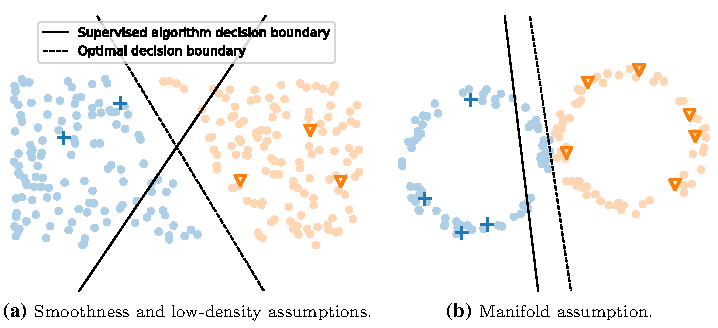
\includegraphics[width=\textwidth]{../img/memoria/3_assumptions.pdf}
\end{figure}


\subsection{Clasificación}

Inicialmente, se pueden diferenciar dos categorías~\cite{engelen2020surveyOnSemiSupervised}: los métodos inductivos, cuyo objetivo principal es construir un clasificador que genere predicciones para cualquier entrada y los métodos transductivos, cuyo poder de predicción está limitado a los objetos utilizados en la fase de entrenamiento.


\begin{figure}[h]
\caption[Taxonomía de métodos de aprendizaje semisupervisado]{Taxonomía de métodos de aprendizaje semisupervisados. Extraída de \textit{A survey on semi-supervised learning}~\cite{engelen2020surveyOnSemiSupervised}.}
\centering
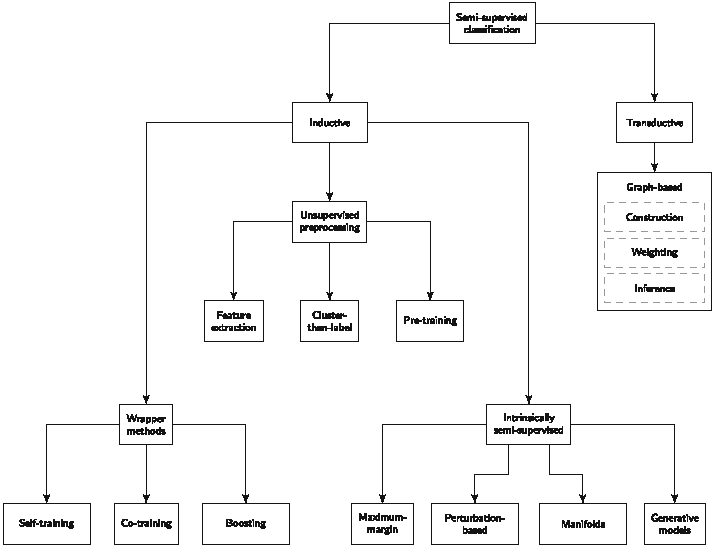
\includegraphics[width=\textwidth]{../img/memoria/3_hoos_taxonomy.pdf}
\end{figure}

Prescindiendo de los métodos transductivos por ser menos versátiles y útiles en nuestro propósito, los métodos inductivos se subdividen en tres grupos~\cite{engelen2020surveyOnSemiSupervised}: \textit{wrapper methods} (o métodos de envoltura), \textit{unsupervised preprocessing} y \textit{intrinsically semi-supervised}, siendo materia de estudio los métodos de envoltura. 


\subsection{Métodos de envoltura}

Estos modelos utilizan uno o más clasificadores que son entrenados iterativamente con los datos etiquetados de entrada, además de con datos pseudo-etiquetados. Se denomina pseudo-etiquetado a aquellos datos que inicialmente no estaban etiquetados, pero acabaron estándolo por iteraciones previas de los clasificadores.

Consecuentemente, el procedimiento consta de dos fases que se repiten en cada iteración: el entrenamiento y el pseudo-etiquetado. Durante el entrenamiento, los clasificadores se alimentan de datos etiquetados (o pseudo-etiquetados). En la fase de pseudo-etiquetado, se utilizan datos no etiquetados para que sean procesados por los clasificadores previamente entrenados. 

Dentro de esta categoría, se pueden diferenciar tres grandes grupos: \textit{self-training}, que utilizan únicamente un clasificador, \textit{co-training}~\cite{engelen2020surveyOnSemiSupervised}, que utilizan más de uno y los \textit{pseudo-labelled boosting methods}, que construyen clasificadores individuales que se alimentan de las predicciones más fiables. Se estudiará más en profundidad los métodos \textit{co-training}.

\subsubsection{Co-training}

En estos algoritmos, varios clasificadores son entrenados iterativamente utilizando datos etiquetados y añadiendo las predicciones (resultados) más confiables al conjunto para ser utilizadas en las siguientes iteraciones~\cite{engelen2020surveyOnSemiSupervised}. Para que los clasificadores sean capaces de generar información distinta, generalmente se divide el conjunto de entrada según alguna característica (no siendo estrictamente necesario). El \textit{co-forest}, algoritmo protagonista de este proyecto, pertenece a esta categoría.

Para que estos métodos tengan éxito, es importante que los clasificadores base no estén fuertemente correlacionados con sus predicciones, ya que entonces se limita el potencial para proporcionar información útil al resto~\cite{engelen2020surveyOnSemiSupervised}. Es decir, los estimadores han de ser diversos. Una de las formas de conseguir diversidad es mediante el uso de clasificadores inestables. Otra, obtener más de una vista del conjunto de datos inicial.


\section{\textit{Ensembles}}

Cuando se cuenta con un único estimador base a la hora de realizar una predicción, la etiqueta asignada es directamente la predicha por el clasificador. Sin embargo, en muchas ocasiones, puede resultar enriquecedor recurrir a lo estimado por más de un modelo~\cite{ensembles2006robi}. 

Se define \textit{ensemble} como un conjunto de modelos de \textit{machine learning} donde cada estimador base genera una predicción individual que se combina con el resto para generar una salida única~\cite{originalCoForest2007}.  Hay varios motivos por los que resulta favorecedor contar con un conjunto de clasificadores en lugar de con un único estimador base~\cite{ensembles2006robi}:

\begin{itemize}
	\item \textbf{Motivos estadísticos:} en muchas ocasiones se obtienen buenos resultados en los datos de entrenamiento, pero un error de generalización alto. También se puede dar el caso en el que un conjunto de clasificadores con resultados similares en el conjunto de prueba actúe de manera distinta en la aplicación real (el conjunto de \textit{test} no es lo suficientemente representativo). En estos casos, el hecho de contar con un conjunto de clasificadores reduce considerablemente las probabilidades de predecir mal una etiqueta. Una analogía en la vida real sería cuando se pide opinión médica a un conjunto de doctores (y no a uno solo) para obtener un diagnóstico no sesgado por las experiencias previas de un sólo médico.
	
	\item \textbf{Gran cantidad de datos:} cuando la cantidad de información es demasiada, puede no ser manejada correctamente por un único clasificador. Por ello, es mejor particionarla en distintos conjuntos de entrenamiento y prueba, y alimentar cada modelo con una partición.
	
	\item \textbf{Escasa cantidad de datos:} si los datos no son suficientes, puede ocurrir que un clasificador no sea capaz de aprender su estructura interna. Por ello, es recomendable realizar un muestreo de los datos (con reemplazo) y entrenar varios modelos distintos con ellos. De esta manera, los errores disminuyen.
	
	\item \textbf{Divide y vencerás:} cuando un problema es demasiado complicado de resolver utilizando un único clasificador, utilizar un conjunto de ellos puede ser efectivo.
\end{itemize}


\subsection{Diversidad y clasificación}

En la realidad, los datos contienen ruido, \textit{outliers}, distribuciones que se solapan, etc. Por ello, es muy complicado obtener un clasificador con un desempeño perfecto~\cite{ensembles2006robi}. Los \textit{ensembles} reducen el error cometido por cada estimador base debido a que combinan las salidas de los mismos. Puede parecer <<negativo>> que los clasificadores individuales difieran. Sin embargo, la realidad es que cuanto más único sea cada estimador utilizado y más distintas sean sus \textit{decision boundaries} (frontera que divide la superficie del problema en partes), mejor.

Esta diversidad se puede obtener de distintas formas, por ejemplo, utilizando distintos conjuntos de entrenamiento y \textit{test} en los estimadores base (utilizando técnicas de \textit{bootstrapping}, por ejemplo). Otra opción muy destacable es utilizando clasificadores <<inestables>> (aquellos que sean muy distintos con pequeños cambios en el conjunto de entrenamiento), como por ejemplo los árboles.

A la hora de crear un \textit{ensemble}, hay dos preguntas clave que realizarse: ¿cómo se van a generar los clasificadores base? ¿cómo van a diferenciarse los unos de los otros?~\cite{ensembles2006robi}.

Para lograr un mayor nivel de diversidad, se pueden utilizar procedimientos de muestreo o selección de parámetros. En función de ellos y de cómo se realice el entrenamiento (consultar imagen~\ref{img:bagging}), los \textit{ensembles} pueden ser de distintos tipos.
	
\subsubsection{\textit{Bagging (Random Forest)}}

El \textit{bagging} es uno de los modelos más antiguos y populares~\cite{ensembles2006robi}. Se compone de un conjunto de estimadores base entrenados en paralelo. Por lo tanto, el resultado es el promedio (o más popular) de las salidas de los modelos simples. Para entrenar cada estimador base se utiliza \textit{bootstrapping}~\cite{engelen2018thesis}, que es una técnica de muestreo que genera un subconjunto de datos seleccionando aleatoriamente muestras de un conjunto mayor permitiendo la repetición. Es decir, los clasificadores son entrenados con un subconjunto aleatorio del total de los datos etiquetados como se ilustra en la figura~\ref{img:bagging}. Esta técnica puede ser utilizada con o sin reemplazo, entendiendo que el muestreo con reemplazo se produce cuando cada una de las unidades maestrales seleccionada es devuelta a la población total antes de extraer la siguiente (puede repetirse).

El \textit{bagging} es muy útil cuando se dispone poca cantidad de datos, y la cantidad de muestras que contiene cada conjunto de entrenamiento es de entre el $75\% - 100\%$ del total del \textit{dataset}~\cite{ensembles2006robi}. Al utilizar \textit{bootstrapping}, los conjuntos de \textit{test} se suelen solapar, además de poder contener muestras repetidas (reemplazo). Por ello, es recomendable utilizar clasificadores base inestables, como por ejemplo los árboles.

Cuando todos los estimadores base son árboles, se habla de \textbf{\textit{random forest}}, uno de los métodos de \textit{bagging} más populares que obtiene resultados certeros debido a la aleatoriedad introducida~\cite{originalCoForest2007}. Cuando el \textit{ensemble} devuelve una etiqueta, es el resultado de una votación realizada por todos los árboles del conjunto. Además de utilizar \textit{bootstrapping}, en el entrenamiento individual de cada árbol, únicamente se <<ven>> algunos atributos (no el total) para introducir mayor aleatoriedad. Es decir, en cada nodo del árbol solo se tienen en cuenta ciertas características seleccionadas aleatoriamente.

\begin{figure}[h]
	\caption[Entrenamiento \textit{bagging} y \textit{boosting}]{Diferencias entre el entrenamiento en \textit{bagging} (izquierda) y \textit{boosting} (derecha).}
	\label{img:bagging}
	\centering
	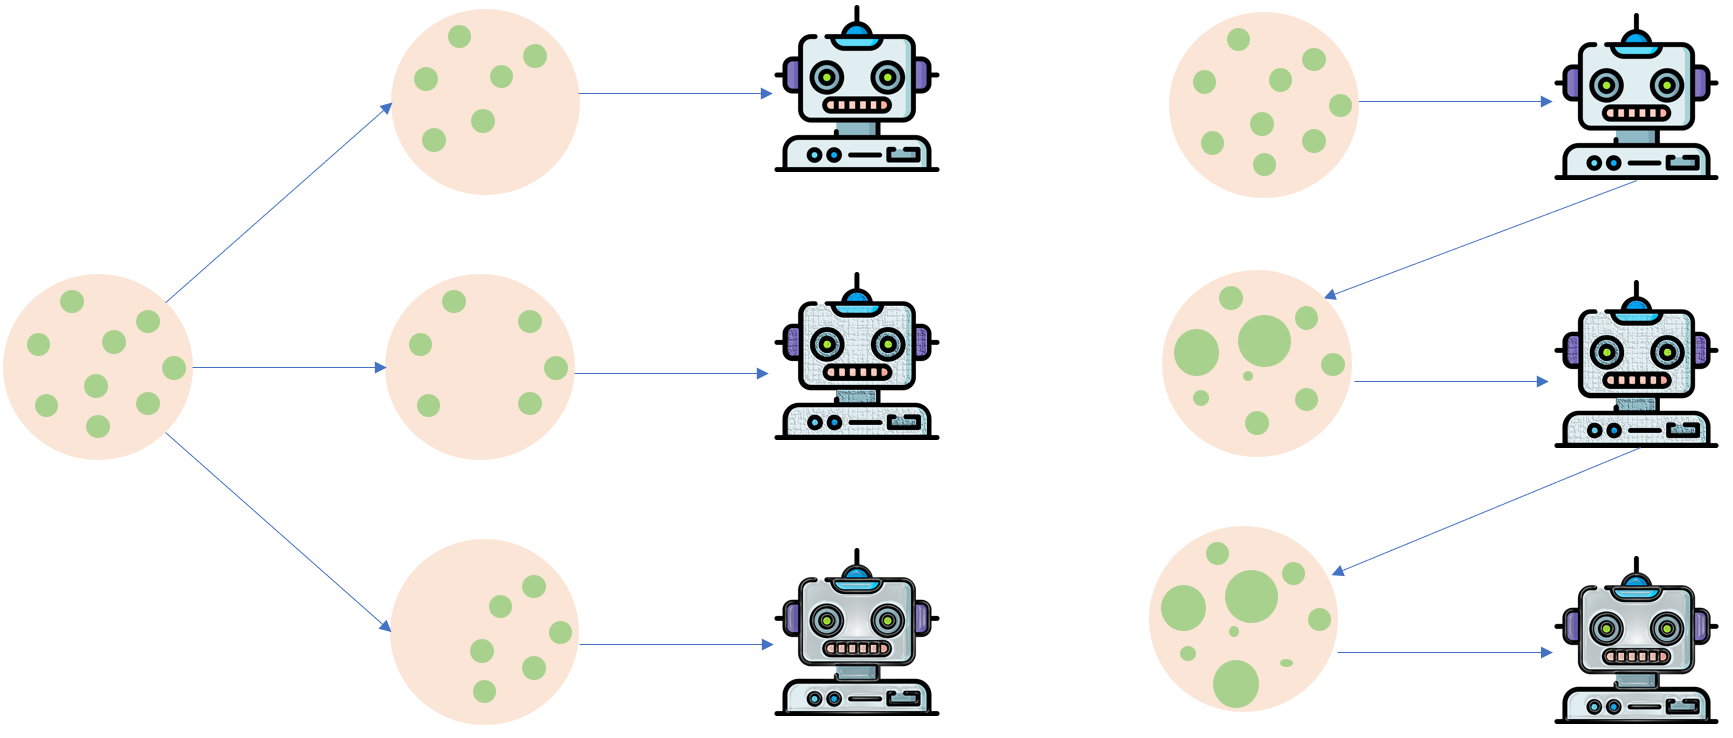
\includegraphics[width=\textwidth]{../img/memoria/3_bagging_boosting}
\end{figure}
	
\subsubsection{\textit{Boosting}}

Si el anterior modelo utiliza los clasificadores base <<en paralelo>>, este lo haría <<en serie>>~\cite{engelen2018thesis}. Es decir, hay un orden secuencial: los estimadores dependen del resultado anterior y tratan de compensar el error que se haya podido cometer (los \textit{weak learners} se convierten en \textit{strong learners}~\cite{ensembles2006robi}).

El entrenamiento se focaliza, por lo tanto, en torno a las instancias que hayan fallado los clasificadores previos. Esto se consigue dando más peso a aquellas muestras mal clasificadas. Por ejemplo, en problemas de regresión, las predicciones con un mayor error cuadrático medio tendrán más peso para el siguiente modelo. En clasificación, los estimadores se entrenan con aquellas muestras en las que los otros elementos del \textit{ensemble} difieran.

\subsection{Combinación de los clasificadores}

Suponiendo que sólo se dispone de las etiquetas asignadas por los clasificadores base como salida, hay diversos modos de <<fusionar>> los \textit{outputs} en uno único~\cite{ensembles2006robi}.

En el caso de que todos los estimadores base sean <<iguales>>, es frecuente utilizar \textit{majority voting} (<<votación de la mayoría>>). Cuenta con tres versiones: la votación unánime (todos los clasificadores coinciden), la mayoría simple (coincidencia de más del $50\%$ de los votos) y la votación por mayoría (la etiqueta que más votos haya recibido, representado en la ilustración~\ref{img:voting}).

Sin embargo, si se sabe que algunos clasificadores son mejores que otros, se puede aplicar \textit{weighted majority voting}, donde las etiquetas predichas por los estimadores con mejor rendimiento tienen más peso que el resto (se asigna una proporción).

\begin{figure}[h]
	\caption[Combinación mediante votación en \textit{ensembles}]{Representación de la combinación mediante votación.}
	\label{img:voting}
	\centering
	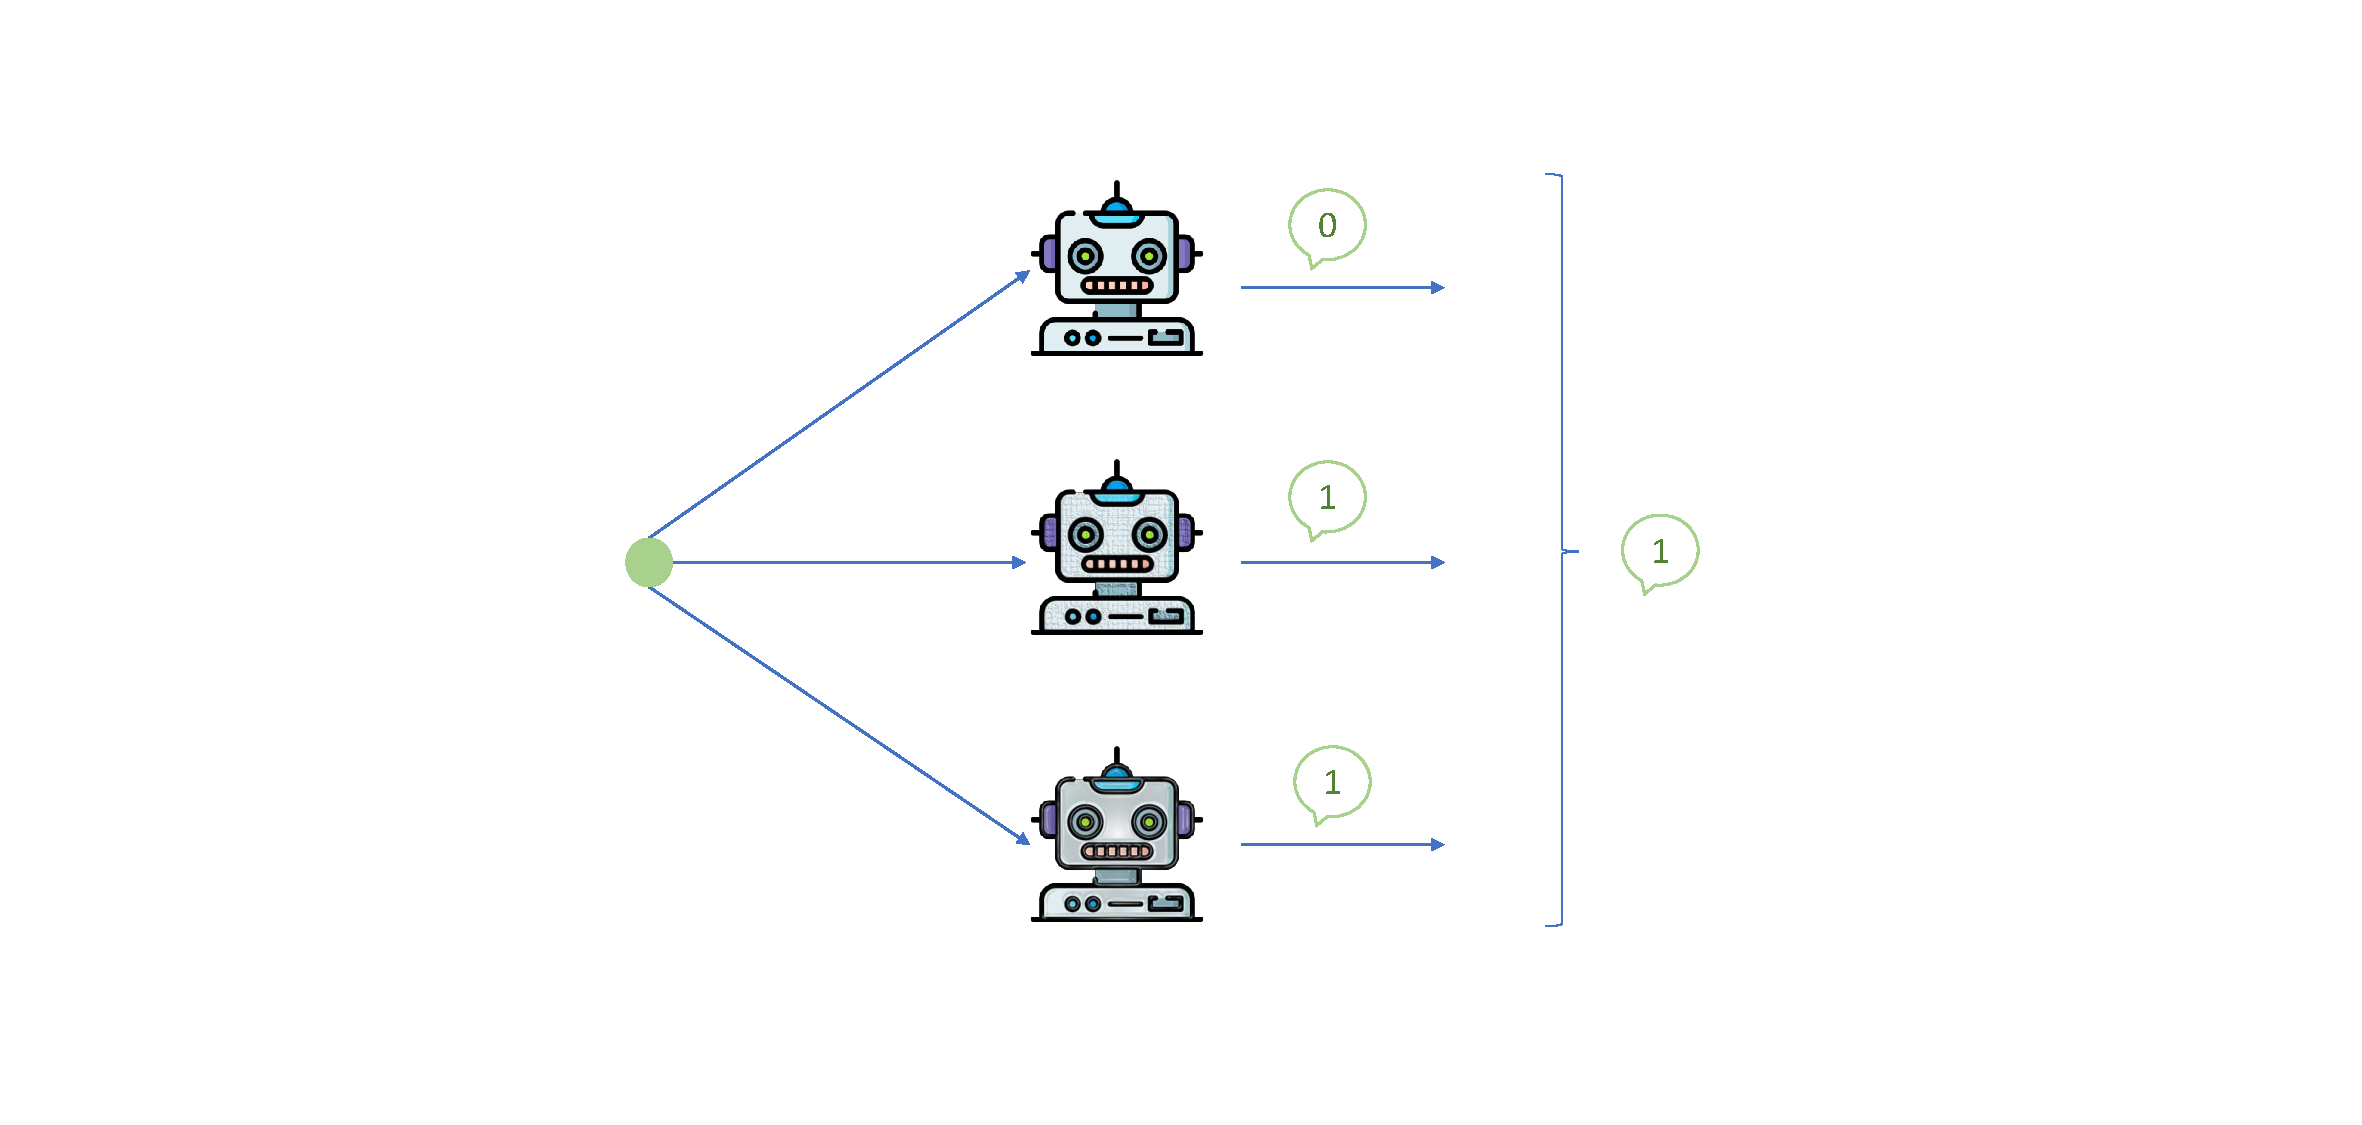
\includegraphics[scale=0.35]{../img/memoria/3_voting}
\end{figure}



\section{Métricas de evaluación}

En este trabajo de investigación se van a realizar continuamente comparaciones entre modelos de clasificación. Para ello, es necesario definir unas métricas. Estas se basan en conceptos que se exponen a continuación~\cite{apuntesSisint}:

\begin{itemize}
	\item \textbf{Verdadero positivo o \textit{True positive}}: se obtiene cuando un clasificador acierta en su predicción y esta es la clase de interés. Generalmente es la clase <<positiva>> y, en el caso de la aplicación en la detección de ataques a sistemas de recomendación, la <<minoritaria>>.
	\item \textbf{Verdadero negativo o \textit{True negative}}: resultado obtenido cuando un clasificador acierta en su predicción y esta no es la clase de interés.
	\item \textbf{Falso positivo o \textit{False positive}}: se obtiene cuando un clasificador falla en su predicción y predice que es la clase de interés, cuando en realidad no lo es.
	\item \textbf{Falso negativo o \textit{False negative}}: resultado obtenido cuando un clasificador falla en su predicción y afirma que una muestra no pertenece a la clase de interés, cuando en realidad sí pertenece.
	
	\item \textbf{Total}: la suma de los cuatro puntos anteriores equivale al total de predicciones ($T = TP + TN + FP + FN$).
	\item \textbf{\textit{Class imbalance problem}}: es un problema que se genera cuando hay muy pocas instancias positivas en el conjunto de datos en comparación con las negativas (es decir, cuando hay un desequilibro evidente entre ambas clases). Generalmente, causa que la \textit{accuracy} (consultar ecuación~\ref{eqn:accuracy}) sea muy elevada, pero no se detecten instancias de la clase positiva, generando modelos inservibles.
\end{itemize}

Dadas las definiciones anteriores, se facilitan las siguientes métricas utilizadas~\cite{apuntesSisint}:

\begin{itemize}
	\item \textbf{\textit{Accuracy}, exactitud o porcentaje de acierto}: mide la tasa de aciertos de un determinado clasificador. A lo largo del proyecto, también es llamada <<\textit{score}>>.
	
	\begin{equation}\label{eqn:accuracy} Accuracy = \frac{|Aciertos|}{|Total|} = \frac{TP + TN}{TP + TN + FP + FN} \end{equation}
	
	\item \textbf{\textit{Error rate}, o porcentaje de error}: mide la tasa de error del clasificador.
	
	\begin{equation}\label{eqn:error} Error Rate = \frac{|Fallos|}{|Total|} = \frac{FP + FN}{TP + TN + FP + FN} = 1 - Accuracy \end{equation}
	
	\item \textbf{Precisión}: mide cuántas predicciones son verdaderamente positivas entre todas las seleccionadas como tal.
	
	\begin{equation}\label{eqn:precision} Precision = \frac{TP}{TP + FP}\end{equation} 
	
	\item \textbf{\textit{Recall}, \textit{sensitivity} o TPR (\textit{true positive rate})}: determina la capacidad del clasificador para detectar clases positivas. En otras palabras, determina el porcentaje de positivos detectados sobre el total de positivos reales.
	
	\begin{equation}\label{eqn:recall} Recall = \frac{TP}{TP + FN}\end{equation}
	
	\item \textbf{\textit{FPR (false positives rate)}}: determina cuántos negativos son clasificados como positivos sobre el total de negativos.
	
	\begin{equation}\label{eqn:FPR} FPR = \frac{FP}{FP + TN}\end{equation}
		
	\item \textbf{\textit{Specificity}}: determina cuántos elementos negativos son detectados.
	\begin{equation}\label{eqn:specificity} Specificity = \frac{TN}{TN + FP}\end{equation}
	
	
	\item \textbf{\textit{F-Measure}}: medida que combina la \textit{precision} y el \textit{recall}. Es de interés puesto que la meta general suele ser maximizar estas dos medidas.
	
	\begin{equation}\label{eqn:f-measure} \textrm{F-Measure} = 2 \times \frac{precision \times recall}{precision + recall} = \frac{ 2 \times TP}{2 \times TP + FP + FN} \end{equation}
	
	\item \textbf{Curva \textit{ROC} (\textit{operating characteristic curve})}: Representación gráfica del \textit{recall} frente a la \textit{specificity}~\cite{AUC2022google}. Un clasificador perfecto tendría una <<curva>> equivalente a un punto en la esquina superior izquierda de la gráfica, mientras que el peor clasificador (uno aleatorio) obtendría una recta diagonal. Si la curva está por debajo de esta recta que divide el área en dos, significa que las predicciones están siendo <<invertidas>>. Esta medida es popular debido a que no se ve afectada por problemas de clases no balanceadas~\cite{AUC2020imbalanced}. Sin embargo, sí que es sensible cuando hay muy pocas instancias positivas en el \textit{dataset} y las estimaciones pueden no ser certeras~\cite{leaningImbalanced2018Salvador}.
	
	\begin{figure}[h]
		\caption[Curva ROC]{Calidad del clasificador en función de su curva \textit{ROC} \footnote{ https:\/\/ca.wikipedia.org\/wiki\/Fitxer:Roc\_curve.svg }. }
		\label{img:curva_roc}
		\centering
		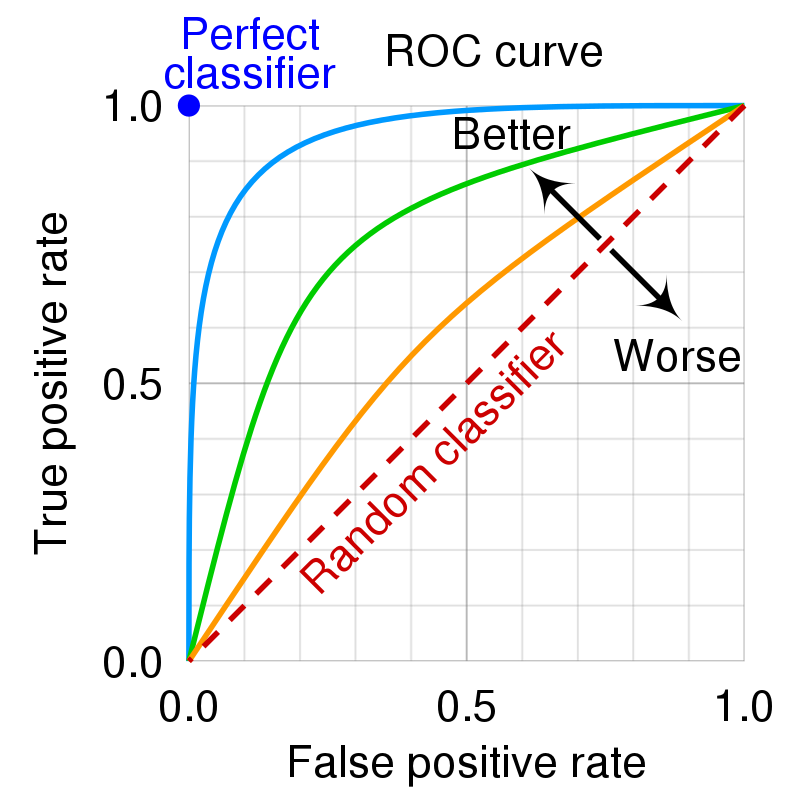
\includegraphics[scale=0.27]{../img/memoria/3_curva_roc}
	\end{figure}

	\item \textbf{Curva \textit{PR} (\textit{precision-recall curve)}}:  Representación gráfica de la precisión frente al \textit{recall}. Cuando se presenta un \textit{class imbalance problem} con muy pocas clases positivas, es adecuado utilizar una curva de estas características debido a que la \textit{precision} y el \textit{recall} permiten evaluar la actuación del clasificador en la clase minoritaria~\cite{imbalanced2013Haibo}.
	
	\item \textbf{\textit{AUC} (\textit{area under curve})}: Número decimal que representa el área bajo una determinada curva. Cuando una curva es perfecta (ya sea \textit{ROC} o \textit{PR}), su área es $1$.
	
	\begin{figure}[h]
		\caption[AUC curvas ROC y PR]{Representación de las curvas \textit{ROC} y \textit{PR} junto con el \textit{AUC} obtenido por cada una para un \textit{co-forest} entrenado con un \textit{dataset} binario.}
		\label{img:curva_roc_pr}
		\centering
		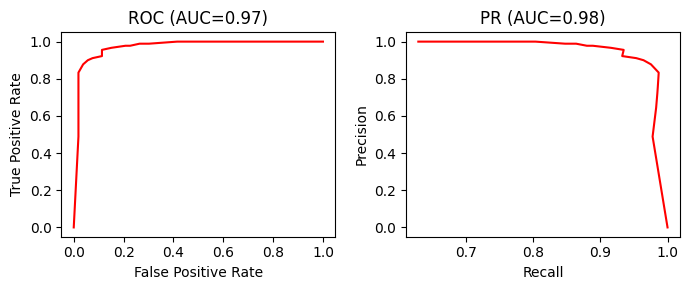
\includegraphics[scale=0.7]{../img/memoria/3_auc_roc_pr}
	\end{figure}
	
\end{itemize}












\section{\textit{Co-forest}}

\subsection{Descripción}

El denominado \textit{co-forest}~\cite{originalCoForest2007} es un método de clasificación para aprendizaje semisupervisado (más concretamente, de envoltura) que permite construir un \textit{ensemble} de árboles de decisión (clasificación). Este método está basado en el \textit{random forest} y se podría considerar su <<versión semisupervisada>>. 

Que sea un algoritmo semisupervisado implica que, durante la fase de entrenamiento, además de utilizar el conjunto de datos etiquetados ($L$), se utilicen también aquellas pseudo-etiquetas de las predicciones con mejor confianza del conjunto de datos no etiquetados ($U$).

El proceso de entrenamiento se realiza iterativamente~\cite{engelen2018thesis}, y en cada una de estas repeticiones, se examina cada árbol y se entrena individualmente con un subconjunto de $L$ ($L_{i}$) y con un subconjunto de $U$ ($L'_{i,t}$) formado por aquellas pseudo-etiquetas que, además de pertenecer a la submuestra (aleatoria), posean un nivel de confianza superior a un umbral definido por el usuario ($\theta$). Quienes estiman esta confianza de predicción para las muestras seleccionadas son el conjunto de todos los árboles que forman el \textit{ensemble} menos el árbol que está siendo entrenado individualmente (de ahora en adelante \textit{concomitant ensemble} o conjunto concomitante).

El criterio de parada de la fase de entrenamiento del \textit{co-forest} es el \textit{out-of-bag error}~\cite{zhou2021SemisupervisedRecommendationAttack} (de ahora en adelante, OOBE). Se define OOBE como el error que comete el conjunto concomitante de un árbol para el total de los datos etiquetados. Es decir, el número de árboles que aciertan la etiqueta entre el número de árboles que votan teniendo en cuenta que, para calcular el OOBE del total de los datos etiquetados, sólo votan aquellos árboles que no hayan utilizado la muestra concreta de $L$ para su entrenamiento.


\subsection{Algoritmo}


\subsubsection{Variables utilizadas}

Para facilitar la comprensión del pseudocódigo, se definen a continuación algunas de las variables utilizadas:
\begin{itemize}
	\item $n$: número total de árboles del ensemble.
	\item $h_{i}$: árbol i-ésimo del conjunto.
	\item $H_{i}$: \textit{concomitant ensemble} o conjunto concomitante del árbol i-ésimo (todos los árboles del \textit{co-forest} menos él).
	\item $x_j$: muestra j-ésima (generalmente sin etiqueta).
	\item $H_i(x_j)$: etiqueta asignada por $H_i$ a la muestra j-ésima.
	\item $w_{i,t,j}$: confianza de predicción (individual) calculada para una muestra $x_j$ por $H_{i}$ en la iteración $t$. Se define confianza como el grado de acuerdo que existe en una votación. 
	\item $W$: sumatorio de las confianzas de predicción individuales de un conjunto $W = \sum w_{i,t,j}$.
	\item $L$: conjunto de datos etiquetados utilizados durante el entrenamiento.
	\item $L_{i}$: subconjunto obtenido tras aplicar \textit{bootstrapping} a $L$ que se utiliza para entrenar el árbol $h_{i}$.
	\item $U$: conjunto de datos no etiquetados utilizados durante el entrenamiento.
	\item $U'_{i,t}$: subconjunto aleatorio de U cuya $W$ es menor que $W_max$ (consultar ecuación~\ref{eqn:Wmax}).
	\item $L'_{i,t}$: subconjunto formado por aquellas muestras de $U'_{i,t}$ cuya confianza de predicción es superior a $\theta$.
	\item $\theta$: nivel de confianza mínimo que tiene que tener el clasificador al predecir la etiqueta de una muestra de $U$ para ser utilizada durante el entrenamiento de un árbol.
	\item $\hat{e}_{i,t}$: OOBE cometido por $H_{i}$ en $L$ en el instante de tiempo $t$.
\end{itemize} 

\subsubsection{Pseudocódigo}

Se facilita a continuación (pseudocódigo~\ref{alg:co-forest}) la versión del \textit{co-forest} de la tesis de Engelen~\cite{engelen2018thesis}, basada en la original~\cite{originalCoForest2007}, pero introduciendo los cambios observables en la sección <<Discusión de los parámetros del algoritmo>>.

\begin{algorithm}
	\KwIn{Conjunto de datos etiquetados $L \lbrace\left(x_i, y_i\right)\rbrace_{i=1}^l$, conjunto de datos no etiquetados $U \lbrace x_i \rbrace_{i=l+1}^{k}$, número de árboles $n$ y umbral de confianza $\theta$}
	\KwOut{\textit{Ensemble} de árboles entrenado $H$.}
	\BlankLine
	\For{$i$ = 0, ..., $n-1$}{
		$L_{i} \leftarrow$ \textit{Bootstrap}($L$)\\
		$h_i$ = EntrenarArbol($L_{i}$)\\
		$\hat{e}_{i,t} \leftarrow 0.5$\\
		$W_{i,0} \leftarrow min(\frac{1}{10}|$U$|, 100)$\\
	}

	$t \leftarrow 0$\\
	\While(){Algún árbol reciba pseudo-etiquetas}{
	$t \leftarrow t + 1$\\
	
	\For{$i$ = 0, ..., $n-1$}{
		$\hat{e}_{i,t} \leftarrow$ OOBE($H_i, L$)\\
		$L'_{i,t} \leftarrow \emptyset$\\
		
		\If{$\hat{e}_{i,t} < \hat{e}_{i,t-1}$}{
			$W_{max} = \hat{e}_{i,t-1}W_{i,t-1}/\hat{e}_{i, t}$\\
			$U'_{i,t} \leftarrow$ Submuestrear($U, H_i, W_{max}$)\\
			$W_{i,t} \leftarrow 0$
			
			\ForEach{$x_j \in U'_{i,t}$}{
				
				\If{Confianza($H_i, x_j$) > $\theta$}{
					$L'_{i,t} \leftarrow L'_{i,t} \cup {x_j, H_i(x_j)}$\\
					$W_{i,t} \leftarrow W_{i,t} + Confianza(H_i, x_j)$
				}
			}
		}
	}
	\For{$i$ = 0, ..., $n-1$}{
		\If{$(e_{i,t} * W_{i,t} < e_{i, t-1} * W_{i, t-1})$}{
			$h_i$ = EntrenarArbol($L_{i} \cup L'_{i,t}$)\\
		}
	}
}
	\Return{$H$}

	\caption{\textit{Co-Forest}}\label{alg:co-forest}
	\end{algorithm}

\subsubsection{Fases}

En primer lugar, se ha de construir un \textit{random forest} de $n$ árboles. Para introducir aleatoriedad, cada uno de esos árboles es entrenado utilizando un subconjunto aleatorio de $L$. Es decir, un subconjunto obtenido tras aplicar \textit{bootstrap} a $L$.

Otro parámetro a tener en cuenta es el número de atributos a considerar en cada árbol de decisión. Por defecto, se ha establecido este valor al $log_{2}$ del total (heurística de Breiman~\cite{engelen2018thesis}). Sin embargo, también podría ser el la raíz cuadrada del total o el total, entre otros.

La segunda fase es entrenar el \textit{random forest} de manera semisupervisada e iterativa hasta que se cumpla el criterio de parada (como se ha mencionado anteriormente, basado en el OOBE). Para ello, se calcula el OOBE de un árbol para una iteración. Si es superior al anterior, se considera que el rendimiento ha empeorado para ese árbol. El algoritmo finaliza cuando todos los árboles empeoran su rendimiento en una determinada iteración.

Por el contrario, en caso de que se haya mejorado, se toma una submuestra de $U$ para pseudo-etiquetar (evidentemente, distinta para cada árbol). Posteriormente se examina cada una de las muestras que forman $U'_{i, t}$, y en caso de que el nivel de confianza supere el umbral, se selecciona esa muestra para el entrenamiento (pasa a formar parte de $L'_{i, t}$).

El último paso sería reentrenar los árboles que hayan cambiado con su propio conjunto inicial de datos etiquetados unido a las pseudo-etiquetas generadas en la correspondiente iteración ($L_{i}\cup L'_{i,t}$). Es decir, en cada iteración se considera $U$ al completo para poder generar la muestra con la que se pseudo-etiquete, y las anteriores pseudo-etiquetas para un árbol en concreto son descartadas~\cite{engelen2018thesis}.


\subsection{Tratamiento del ruido y teoría de errores}

Como se señala en el \textit{paper} de Zhou y Duan~\cite{zhou2021SemisupervisedRecommendationAttack}, de acuerdo con el trabajo de Angluin y Laird~\cite{noisyExamplesCoforest1988Dana}, si el tamaño de los datos utilizados en el entrenamiento ($m$), la tasa de ruido ($\eta$), el error de la hipótesis en el peor caso ($\epsilon$) y una constante ($c$) cumplen la relación de la ecuación~\ref{eqn:rel_convergencia_hipotesis}, entonces la hipótesis aprendida por el árbol $h_{i}$ (que minimiza el desacuerdo en un conjunto de muestras de entrenamiento con ruido) converge a la hipótesis verdadera.

\begin{equation}\label{eqn:rel_convergencia_hipotesis} m = \frac{c}{\epsilon^{2}(1-2\eta)^{2}} \end{equation} 

De acuerdo con~\cite{zhou2021SemisupervisedRecommendationAttack}, se puede obtener la función de utilidad mostrada en la ecuación~\ref{eqn:operar_rel_convergencia} operando en la expresión~\ref{eqn:rel_convergencia_hipotesis}.

\begin{equation}\label{eqn:operar_rel_convergencia} f = \frac{c}{\epsilon^{2}} = m(1-2\eta)^{2} \end{equation} 

Como se ha mostrado en el pseudocódigo, en la iteración i-ésima un determinado árbol se entrena con sus datos etiquetados $L_{i}$ y un conjunto de pseudo-etiquetas $L'_{i,t}$. Si se considera que el OOBE cometido en $L$ por $H_{i}$ es $\hat{e}_{i,t}$, entonces se puede estimar que el número de pseudo-etiquetas erróneas en $L'_{i,t}$ equivale a $\hat{e}_{i,t} \times W_{i,t}$ (se recuerda al lector que $W_{i,t}$ es el sumatorio de la confianza de predicción (grado de acuerdo) de $H_{i}$ en cada muestra de $L'_{i,t}$). Por lo tanto, la tasa de ruido que se encuentra en $L_{i} \cup L'_{i,t}$ es la estimada por la ecuación~\ref{eqn:ruido_it}, donde $W_0$ y $\eta_0$ son los parámetros correspondientes a $L$. 

\begin{equation}\label{eqn:ruido_it} \eta = \frac{\eta_{0}W_{0} + \hat{e}_{i,t}W_{i,t}}{W_{0} + W_{i,t}} \end{equation} 

De acuerdo con la ecuación~\ref{eqn:operar_rel_convergencia}, la función de utilidad $f$ es inversamente proporcional a $\epsilon^2$. Por lo tanto, si se quiere reducir el error cometido, se debe aumentar la utilidad de cada árbol en cada iteración~\cite{zhou2021SemisupervisedRecommendationAttack}. Consecuentemente, se debe cumplir la ecuación~\ref{eqn:relacion_e_W}. 

\begin{equation}\label{eqn:relacion_e_W} \frac{\hat{e}_{i,t}}{\widehat{e}_{i, t-1}} < \frac{W_{i,t-1}}{W_{i,t}} < 1 \end{equation} 


\subsubsection{Discusión acerca de los parámetros del algoritmo}

Intuitivamente se puede deducir la ecuación~\ref{eqn:relacion_e_W}, ya que el error debe disminuir y la confianza de predicción aumentar con cada iteración. Sin embargo, aunque esto se cumpla, puede ser que se deje de cumplir que $\hat{e}_{i,t}W_{i,t} < \hat{e}_{i,t-1}W_{i,t-1}$, ya que puede ocurrir que $ W_{i,t} >>> W_{i,t-1}$. Por este motivo y para cumplir con lo expuesto en la ecuación~\ref{eqn:relacion_e_W}, se limita $W_{max}$ como se muestra en la ecuación~\ref{eqn:Wmax} al realizar el muestreo de $U$ en el algoritmo.

\begin{equation}\label{eqn:Wmax} W_{max} = \frac{\hat{e}_{i,t-1}W_{i,t-1}}{\hat{e}_{i, t}} > W_{i,t} \end{equation}


\label{parag:Wmax_inicial} El algoritmo original propuesto por~\cite{originalCoForest2007} y el utilizado en~\cite{zhou2021SemisupervisedRecommendationAttack} dejan, sin embargo, una cuestión pendiente. Como se puede observar en la ecuación~\ref{eqn:Wmax}, $W_{max}$ requiere para calcularse tanto el OOBE como la $W$ obtenida en la iteración anterior, y ambos autores inician $W$ a 0. Esto implica que en la primera iteración $W_{max} = 0$ y, por lo tanto, evita que se realice un muestreo de $U$ para pseudo-etiquetar (pararía el algoritmo). En su tesis, Engelen~\cite{engelen2018thesis} propone solucionar este problema iniciando $W = min(\frac{1}{10}|U|, 100)$, aunque destaca que imponer esta constante hace que el impacto de los datos sin etiquetar en el algoritmo dependa profundamente del tamaño del \textit{dataset}.


\subsubsection{Decisiones de implementación}

Además de los aspectos expuestos en el apartado anterior, hay dos decisiones adicionales que se han tomado en la implementación por no estar contempladas en el algoritmo original.

En primer lugar, el valor de $W_{max}$ cuando $\hat{e}_{i, t}$  es $0$. Como se puede comprobar en la fórmula~\ref{eqn:Wmax}, al estar en el denominador, se produce una indeterminación. Si el valor se sustituye por un número muy cercano a 0, $W_{max}$ tiende a infinito, provocando una submuestra de U ilimitada. Como la función de $W_{max}$ es determinar el tamaño de la submuestra, y en este caso el error del conjunto concomitante es nulo, se ha decidido mantenerlo alto pero limitar a $\theta\times|U|$.

Por otro lado, tampoco se hace explícito cómo iniciar $W_{i,t}$ en aquellas iteraciones en las que no se cumple que $\hat{e}_{i,t} < \hat{e}_{i,t-1}$. Se puede pensar que se debe iniciar a 0. Sin embargo, esto causaría que en iteraciones posteriores nunca se genere una submuestra de U, pues como se puede comprobar en la ecuación~\ref{eqn:Wmax} el tamaño de $W_{max}$ sería $0$. Por este motivo, se ha decidido iniciar $W_{i,t} \leftarrow W_{i,t-1}$.


\section{\textit{Tri-Training}}

\subsection{Descripción}


El denominado \textit{tri-training}~\cite{tritraining2005@original} es un método de clasificación para aprendizaje semisupervisado perteneciente a la rama del \textit{co-training}. Utiliza tres estimadores base ($i$, $j$ y $k$) que son entrenados utilizando un conjunto de datos etiquetados $L$ y pseudo-etiquetas generadas por el resto del conjunto.

Dos de las principales características que lo convierten en un algoritmo fácil de utilizar en escenarios reales de minería de datos es que no requiere vistas suficientes y redundantes de los datos ni el uso de distintos algoritmos de aprendizaje supervisado en los clasificadores base~\cite{tritraining2005@original}. Sin embargo, sí que es un requisito que los estimadores base sean diversos.

El proceso de entrenamiento se realiza iterativamente, actualizando los estimadores base oportunos utilizando $L$ y un subconjunto de $U$ ($L_i$) pseudo-etiquetado por los dos clasificadores restantes. Este subconjunto se genera (para $i$) utilizando aquellas instancias de $U$ en las que los estimadores concomitantes de $i$ (es decir, $j$ y $k$) concuerden en su etiqueta.

Por otro lado, el error para $i$ se aproxima dividiendo el número de muestras de $L$ para las cuales el conjunto concomitante de $i$ realiza una predicción incorrecta entre el número total de muestras de $L$ para las cuales la etiqueta predicha por $j$ es la misma que la predicha por $k$.

\subsection{Algoritmo}

\subsubsection{Variables utilizadas}

Para facilitar la comprensión del pseudocódigo, se definen a continuación algunas de las variables utilizadas:

\begin{itemize}
	\item $h_{i}$: estimador i-ésimo del \textit{ensemble} (entrenado con un conjunto concreto de datos que puede variar en cada iteración).
	\item $L$: conjunto de datos etiquetados utilizados durante el entrenamiento.
	\item $U$: conjunto de datos no etiquetados utilizados durante el entrenamiento.
	\item $S_{i}$: subconjunto obtenido tras realizar \textit{bootstrap} a $L$ para un clasificador en concreto.
	\item $L_{i}$: subconjunto de $U$ pseudo-etiquetado para $i$.
	\item $l'_{i}$: tamaño del conjunto $L_i$ en la iteración anterior (utilizable para saber si anteriormente un clasificador ha sido entrenado con pseudo-etiquetas o no).	
	\item $e_{i}$: error del estimador $i$.	
	\item $e'_{i}$: error anterior del clasificador $i$.	
\end{itemize} 

\subsubsection{Pseudocódigo}
Se facilita a continuación (pseudocódigo~\ref{alg:tri-training}) el pseudocódigo original~\cite{tritraining2005@original} del \textit{tri-training}.

\begin{algorithm}
	
	\KwIn{Conjunto de datos etiquetados $L$, conjunto de datos no etiquetados $U$, tres clasificadores base.}
	\KwOut{\textit{Ensemble} de tres estimadores base entrenados.}
	\BlankLine
	
	\For{$i$ = 1, ..., 3}{
		$S_{i} \leftarrow$ \textit{Bootstrap}($L$)\\
		$h_i \leftarrow$ EntrenarClasificador($S_{i}$)\\
		${e'}_{i} \leftarrow$ 0.5\\
		${l'}_{i} \leftarrow$ 0.0\\
	}
	
	\While(){Algún estimador base reciba pseudo-etiquetas}{
		\For{$i$ = 1, ..., 3}{
			$L_{i} \leftarrow \emptyset$\\
			$actualizar_i \leftarrow$ Falso\\
			${e}_{i} \leftarrow Error(h_i \& h_k) (j, k \ne i)$
			
			\If{${e}_{i} < {e'}_{i}$}{
				\ForEach{$x \in U$}{
					\If{$h_j(x) = h_k(x)$ $(j, k \ne i)$}{
						$L_{i} \leftarrow L_{i} \cup \{(x, h_j(x))\}$\\
					}
				}
				
				\If{$l'_i = 0$} {
					$l'_i \leftarrow \lfloor \frac{e_i}{e'_i - e_i} + 1  \rfloor$
				}
				
				\If{$l'_i < |L_i|$} {
					\If{$e_i \times |L_i| < e'_i \times l'_i$} {
						$actualizar_i \leftarrow$ Verdadero\\
					}
					\ElseIf{ $l'_i > \frac{e_i}{e'_i - e_i}$} {
						$|L_i| \leftarrow Submuestrear(L_i, \lceil \frac{e'_i \times l'_i}{e_i} - 1\rceil)$\\
						$actualizar_i \leftarrow$ True\\
					}
				}
			}
		}
		
		\For{$i$ = 1, ..., $3$}{
			\If{$actualizar_i \leftarrow$ True\\}{
				$h_i$ = Entrenar($L \cup L_{i}$)\\
				$e'_i \leftarrow e_i$\\
				$l'_i \leftarrow |L_i|$\\
			}
		}
	}
	\caption{\textit{Tri-Training}}\label{alg:tri-training}
\end{algorithm}

\subsubsection{Fases}

En primer lugar, se entrenan los estimadores base utilizando un subconjunto aleatorio de $L$.

La segunda fase es entrenar el \textit{tri-training} de manera semisupervisada e iterativa hasta que los estimadores base no reciban nuevas etiquetas del resto del \textit{ensemble}. Para ello, se comprueba que el error (explicado anteriormente) sea menor que en la iteración anterior, y en ese caso, se genera $L_i$ utilizando aquellas instancias de $U$ en las que los estimadores concomitantes de $i$ (es decir, $j$ y $k$) concuerden en su etiqueta. En caso de que anteriormente no se haya entrenado con pseudo-etiquetas, se estima el valor que hubiese tenido el conjunto $L_i$ anterior.

Posteriormente, se comprueba si el conjunto $L_i$ nuevo es mayor que el anterior. En caso de que lo sea, se realizan algunas correcciones para evitar violar ecuaciones relacionadas con el tratamiento de errores. Puede llegar a ocurrir que se reduzca el tamaño de $L_i$ durante este proceso.

El último paso sería reentrenar los clasificadores base que hayan recibido nuevas etiquetas con estas mismas unidas a $L$.

\subsection{Tratamiento del ruido y teoría de errores}

En este algoritmo, no es necesario calcular explícitamente la <<confianza>> del conjunto para cada muestra de $U$ debido a que, para que se añada a $L_i$, es suficiente con que los otros dos estimadores base del conjunto coincidan en la etiqueta~\cite{tritraining2005@original}. Puede ocurrir que tanto $j$ como $k$ se equivoquen en una predicción y, por lo tanto, se añada ruido al conjunto de entrenamiento de $i$. Sin embargo, como se comentó anteriormente en el \textit{co-forest}, de acuerdo con el trabajo de Angluin y Laird~\cite{noisyExamplesCoforest1988Dana}, si el tamaño de los datos utilizados en el entrenamiento ($m$), la tasa de ruido ($\eta$), el error de la hipótesis en el peor caso ($\epsilon$) y una constante ($c$) cumplen la relación de la ecuación~\ref{eqn:rel_convergencia_hipotesis}, entonces la hipótesis aprendida por el estimador $h_{i}$ converge a la hipótesis verdadera.

Para cada iteración del algoritmo, se considera un $L_i$ independiente y obtenido considerando todo $U$. El ratio del ruido de clasificación en la iteración $t$-ésima se puede calcular mediante la ecuación~\ref{eqn:ruido_it_tritraining}, donde $\check{e}_{1}^{t}$ es el límite superior del error cometido por $j$ y $k$ en la iteración $t$, $L^t$ es el conjunto de pseudo-etiquetas para $i$ en la iteración $t$ y $\eta_L$ es la tasa de ruido en $L$.

\begin{equation}\label{eqn:ruido_it_tritraining} \eta^{t} = \frac{\eta_{L}|L| + \check{e}_{1}^{t}|L^{t}|}{|L \cup L^{t}|} \end{equation} 

Como se muestra en la función de utilidad de la ecuación~\ref{eqn:operar_rel_convergencia}, como $f$ es inversamente proporcional a  $\frac{c}{\epsilon^{2}}$, entonces se puede deducir que si $f^t > f^{t-1}$ entonces $e^t < e^{t-1}$, lo que implica que el clasificador $i$ va a mejorar si se utilizan las pseudo-etiquetas de $L^t$ en el entrenamiento~\cite{tritraining2005@original}.

\section{\textit{Democratic-co learning}}

\subsection{Descripción}

El \textit{democratic-co learning} es un método de aprendizaje semisupervisado que sólo necesita una vista de los datos para entrenarse y, además, es aplicable cuando se tiene un pequeño conjunto de datos etiquetados~\cite{democraticCoLearning2004original}.

Como estimadores base se utiliza un conjunto de algoritmos de aprendizaje que se utiliza para entrenar un conjunto de clasificadores. Teóricamente este conjunto puede tener un tamaño arbitrario ($n$), aunque en aplicaciones reales, $n$ equivale a $3$.

Además, en la fase de predicción, el método cuenta con un algoritmo de combinación de etiquetas basado en el <<peso>> (como sinónimo de confianza) que tiene cada clasificador~\cite{democraticCoLearning2004original}.

\subsection{Algoritmo}

\subsubsection{Variables utilizadas}

Se definen a continuación algunas de las variables utilizadas en el pseudocódigo facilitado por~\cite{democraticCoLearning2004original}:

\begin{itemize}
	\item $A_{i}$: algoritmo de aprendizaje i-ésimo original (antes de ser entrenado).
	\item $H_{i}$: estimador i-ésimo del \textit{ensemble} (entrenado con un conjunto concreto de datos que puede variar en cada iteración).
	\item $L$: conjunto de datos etiquetados utilizados durante el entrenamiento.
	\item $U$: conjunto de datos no etiquetados utilizados durante el entrenamiento.
	\item $L_{i}$: datos etiquetados utilizados para entrenar a $i$.
	\item $L'_{i}$: datos pseudoetiquetados propuestos (pueden ser rechazados) para añadir a $L_i$.
	\item $e_{i}$: estima el número de etiquetas erróneas contenidas en $L_i$.
	\item $e'_{i}$: estima la nueva tasa de error.
	\item $q_{i}$: estima la tasa de error.
	\item $q'_{i}$: estima la nueva tasa de error si se añade $L'_i$ a $L_i$.
	\item $c_{j}$:  conjunto de estimadores que concuerdan en que la etiqueta para una muestra $x$ es $j$.
	\item $l_i, h_i$: límites inferior y superior del intervalo de confianza al 95\% para el estimador $H_i$.
	\item $w_i$: peso asociado al estimador $H_i$. Es el valor que estima la <<confianza>> que se tiene en un determinado clasificador base.
\end{itemize} 

\subsubsection{Pseudocódigo}

Se facilita a continuación (pseudocódigo~\ref{alg:democratic-co}) el pseudocódigo original~\cite{democraticCoLearning2004original} del \textit{democratic-co learning}.

\begin{algorithm}
	\KwIn{Conjunto de datos etiquetados $L$, conjunto de datos no etiquetados $U$, clasificadores base ($A_1, ..., A_n$).}
	\KwOut{\textit{Ensemble} entrenado.}
	\BlankLine
	
	\For{$i$ = 1, ..., $n$}{
		${e}_{i}$ = 0.0\\
		${L}_{i} \leftarrow L$\\
	}
	
	\While(){Algún estimador base reciba pseudo-etiquetas}{
		
		\For{$i$ = 1, ..., n}{
			$H_i$ = Entrenar($A_i, L_{i}$)\\ }
		
		\For{$x \in U$}{
			\For{posible etiqueta $j = 1, ..., r$} {
				$c_j = |\{H_i | H_i(x) = j\}|$ }
			$k$ = arg max$_j\{c_j\}$
		}
	
		\# Se escogen las muestras a proponer para etiquetar\\
		\For{$i = 1, ..., n$}{
			$l_i, h_i$ = Intervalo\_de\_confianza\_95\%($H_i, L$)\\
			$w_i = (l_i + h_i) / 2$\\}
			
		\For{$i = 1,...,n$}
			{$L'_i = \emptyset$}
		
		\If{ $\sum_{H_j(x) = c_k}^{} w_j$ > max$_{c'_k \ne c_k} \sum_{H_j(x) = c'_k}^{}w_j$}
		{$L'_i = L'_i \cup \{(x, c_k)\}, \forall i$ tal que $H_i(x) \ne c_k$}
		
		\# Se estima si añadir $L'_i$ a $L_i$ mejora la \textit{accuracy}\\
		\For{$i = 1,...,n$}{
			$l_i, h_i$ = Intervalo\_de\_confianza\_95\%($H_i, L_i$)\\
			$q_i = |L_i| (1-2(\frac{e_i}{|L_i|}))^2$\\
			$e'_i = (1-\frac{\sum_{i=1}^{d}l_i}{d}) |L'_i|$\\
			$q'_i = |L_i \cup L'_i| (1-\frac{2 (e_i + e'_i)}{|L_i \cup L'_i|})^2$\\
			
			\If{$q'_i$ > $q_i$}{
				$L_i = L_i \cup L'_i$\\
				$e_i = e_i + e'_i$
			}
		}
	}

	\caption{\textit{Democratic-co}}\label{alg:democratic-co}
\end{algorithm}

\subsubsection{Fases}

Durante el entrenamiento se pueden diferenciar distintas fases. De manera similar a otros algoritmos, el criterio de parada es que ningún clasificador reciba nuevas pseudoetiquetas (Es decir, ningún $L_i$ cambia).

En cada iteración se entrena cada clasificador base con su conjunto de datos etiquetados (formado por $L$ y pseudoetiquetas de iteraciones anteriores). Posteriormente, para cada muestra contenida en $U$, se genera un <<grupo>> que contiene aquellos clasificadores que coinciden en la etiqueta predicha para la muestra.

A continuación, se escogen aquellas muestras a añadir a los conjuntos $L'_i$ (es decir, las muestras <<propuestas>>). Es destacable que estas nuevas etiquetas sólo se añaden al conjunto de entrenamiento de los clasificadores que han predicho una etiqueta diferente a la más votada.

Antes de añadir las muestras propuestas al conjunto de entrenamiento de los clasificadores de forma definitiva se estima si, con este nuevo cambio, se mejora la \textit{accuracy}, y sólo se realiza en caso afirmativo. Este proceso se repite hasta cumplir el criterio de parada.

\subsection{Combinación de los resultados y corrección de errores}

Aunque la forma más simple de crear la hipótesis final es combinando mediante votación por mayoría, el \textit{democratic-co learning} tiene en cuenta, además, la confianza individual que se tiene en cada clasificador ($w_i$) a la hora de realizar la predicción global.

De este modo, se dividen los clasificadores en grupos dependiendo de la etiqueta a la que hayan votado y se calcula la confianza media que se tiene en cada grupo. Para ello, además, se utiliza una corrección de \textit{Laplace} (de la forma $s=\frac{n+0.5}{n+1}$) para evitar el sesgo generado cuando se tiene un grupo muy pequeño~\cite{democraticCoLearning2004original}.

Debido a que este ajuste puede no resultar efectivo cuando los valores de confianza individuales para cada clasificador son muy dispares, se ignoran aquellos clasificadores con $w$ < 0.5 (consultar algoritmo~\ref{alg:democratic-co-combination}).

\begin{algorithm}
	
	\KwIn{Conjunto de instancias a predecir.}
	\KwOut{Conjunto de etiquetas predichas.}
	\BlankLine
	
	\For{$x$ perteneciente a las instancias a predecir}{
		\For{i = 1,...,n}{
			\If{$H_i(x)$ predice la etiqueta $c_j$ y $w_i$ > 0.5}{
				$G_j = G_j \cup \{H_i\} $\\
			}
		}
	
		\For{j = 1,...,r}{
			$\overline{C}_{G_j} = \frac{|G_j| + 0.5}{|G_j| + 1} \times \frac{\sum_{H_i \in G_j}^{}w_i}{|G_j|}$
		}
	
		$H$ predice con $G_k$ para toda $k$ = argmax$_j(\overline{C}_{G_j})$
	}
	\caption{\textit{Combinación del \textit{democratic-co learning}}}\label{alg:democratic-co-combination}
\end{algorithm}


\section{Conceptos básicos de ciberseguridad}

\subsection{Sistemas de cifrado}

Un sistema de cifrado es un algoritmo que convierte un texto plano (\textit{input}) en un texto cifrado (\textit{output}). La clave reside en que el nuevo texto es ilegible si se carece de la clave necesaria para descifrarlo, y debe ser lo suficientemente seguro como para que romperlo requiera una cantidad extremadamente grande de recursos (generalmente, tiempo)~\cite{cifradoAvast}. El cifrado es aplicable a datos almacenados o <<en movimiento>> (por ejemplo, intercambio de datos a través de internet).

\subsubsection{Cifrado simétrico o criptografía de clave privada}

En este tipo de algoritmos, la clave de cifrado y descifrado es la misma (de ahí que deba permanecer <<privada>>). Se conocen dos tipos, los cifrados de bloque y los cifrados de flujo~\cite{apuntesCybersec}.

En los cifrados de bloque, el texto se divide en bloques de una longitud fija y se cifran bloque a bloque. En función de los modos de operación (los más comunes ECB, CBC, OFM y CTR), también se pueden variar las propiedades de los algoritmos. Algunos de los ejemplos más comunes son DES, Triple DES, AES o \textit{Twofish}.

\subsubsection{Cifrado asimétrico o criptografía de clave pública}

En este tipo de sistemas, se utiliza una clave para cifrar los datos (la clave pública) y otra distinta para descifrarlos (la clave privada)~\cite{cifradoIBM}. Generalmente este tipo de cifrado es mucho más costoso computacionalmente~\cite{apuntesCybersec}, por ello no suelen ser utilizados cuando la cantidad de información a procesar es demasiado grande. 

Algunos de los métodos más comunes son RSA o ECC (criptografía de curva elíptica). Dentro de este tipo de algoritmos también se encuentran los sistemas de intercambio de claves, como \textit{Diffie-Hellman}.

\subsection{Peticiones HTTP}

En la programación web, los clientes se comunican con los servidores realizando peticiones mediante el protocolo HTTP. El cliente realiza \textit{requests} (por ejemplo, una petición \textit{get} cuando se quiere solicitar un recurso o una \textit{post} para enviar datos al servidor), mientras que el servidor responde mediante \textit{responses}.

Estas peticiones contienen cabeceras y código de estado. Para el desarrollo de este proyecto, es importante conocer ciertos campos de la cabecera, entre ellos las \textit{cookies} (pueden ser usadas para indicar que se ha iniciado sesión), los \textit{proxies} (o servidores intermedios) y el \textit{user-agent} (información sobre el dispositivo que realiza una consulta). Estos campos pueden ser introducidos mediante código~\cite{httpHeaders}.

Además es destacable el código de estado, ya que permite conocer si una petición ha sido completada con éxito. En concreto, aquellos códigos comprendidos entre el 100 y el 199 son informativos, entre el 200 y el 299 son operaciones exitosas, entre el 300 y el 399 son redirecciones, entre el 400 y el 499 son errores por parte del cliente y entre el 500 y el 599 son errores por parte del servidor~\cite{httpStatus}.





\subsection{Comunicaciones anónimas}

Las redes clásicas son sencillamente rastreables. Póngase un ejemplo: hacer una consulta en internet. En este caso, el ordenador peticionario genera un paquete que circula hasta el \textit{router} de la red a la que esté conectado. Este \textit{router} lo reenvía a los DNS (\textit{domain name service}) del ISP (\textit{internet service provider}) correspondiente, y de ahí puede ir directamente a la página que se desea consultar, o por el contrario pasar por un mayor número de nodos intermedios.

Este camino es relativamente sencillo de rastrear~\cite{TorAndrea2022}, ya que los ISP tienen acceso a los metadatos de las comunicaciones. Adicionalmente, si el contenido de los mensajes se encuentra incorrectamente cifrado, puede derivar en un ataque a los mismos en caso de intercepción por parte de alguno de los nodos intermedios. Se puede pensar que ocultar esta información a terceros es tan sencillo como, por ejemplo, utilizar una de las bien conocidas VPN (\textit{virtual private network}). Sin embargo, los proveedores de servicio de las VPN serán ahora quienes puedan acceder a los metadatos de las comunicaciones~\cite{TorKeepCoding2022}.


\subsubsection{Enrutado cebolla, red Tor y protocolo SOCKS5}

Uno de los protocolos que permite ocultar esta información es el llamado enrutado cebolla (\textit{onion routing})~\cite{TorAvast2022}, que recibe su nombre por el sistema de capas que utiliza, como se representa en la imagen~\ref{img:red_tor}. En el mismo, se pueden diferenciar las siguientes fases~\cite{TorKeepCoding2022}: 

\begin{figure}[h]
	\caption[Enrutado cebolla.]{Infografía de la red Tor y del enrutado cebolla.}
	\label{img:red_tor}
	\centering
	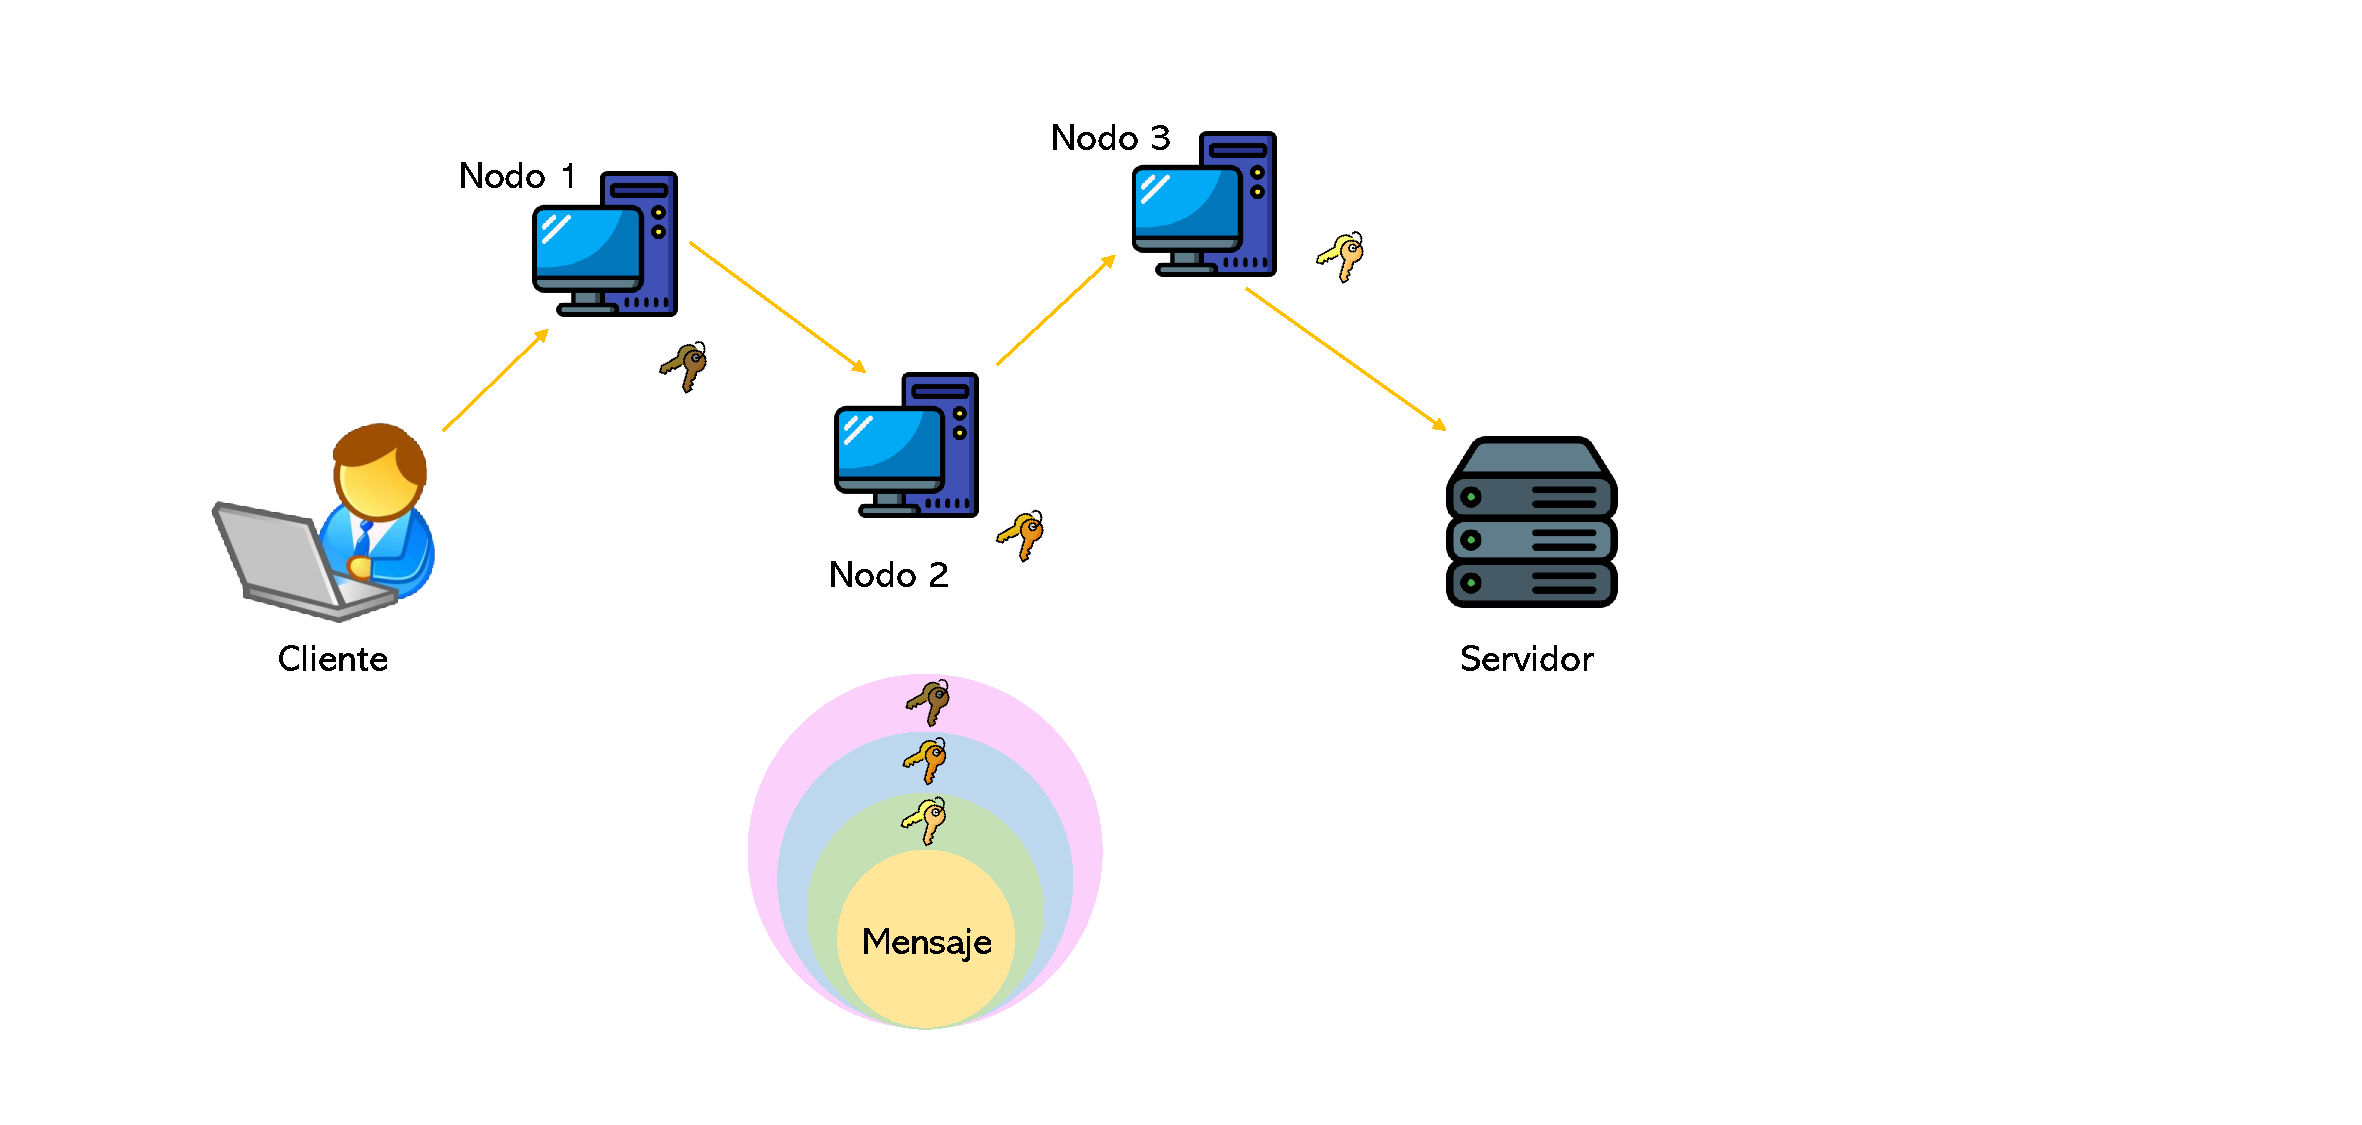
\includegraphics[scale=0.45]{../img/memoria/3_onion_routing}
\end{figure}

\begin{enumerate}
	\item Fase uno: la petición se cifra en varias capas (el estándar es 3). Es decir, con la clave pública del nodo de salida, la del nodo intermedio y, por último, al del nodo de entrada. Recordemos que para descifrar una capa, es necesario la clave privada del nodo correspondiente.
	\item Fase dos: el servidor de entrada recibe la petición cifrada, y se encarga de descifrar la capa externa (posee la clave), obteniendo la dirección IP del nodo intermedio. De este modo, el servidor puede reenviar el mensaje a este último.
	\item Fase tres: el servidor del medio descifra la siguiente capa y encuentra la dirección IP del nodo de salida. Reenvía el resto de la petición cifrada.
	\item Fase cuatro: el servidor de salida descifra la última capa y accede a la petición. Sin embargo, no tiene información acerca de quién la realizo. Sí sabe, en su defecto, la dirección del nodo inmediatamente anterior, por lo que puede resolverla y devolvérsela.
\end{enumerate}

La red Tor, utiliza este sistema~\cite{TorAndrea2022} de enrutado. Para ello, calcula una ruta pseudo-aleatoria hacia destino, obteniendo las claves públicas de los nodos intermedios. Por otro lado, SOCKS5 es un protocolo de Internet usado por Tor~\cite{SOCKS5Tor2022} que permite redirigir el tráfico a través de la red Tor, actuándo como un proxy de la capa de sesión del protocolo OSI. Por motivos de seguridad, se usará más adelante para ocultar la dirección IP de los investigadores a la hora de extraer vectores de características de sitios \textit{phishing}.

\subsection{Ataques web y vulnerabilidades en navegadores}

Cada vez que se visita una web, el navegador (ya sea en ventana o pestaña) carga el contenido, lo renderiza y responde a los eventos. Esto no deja de ser una oportunidad para los atacantes, que pueden utilizar las etiquetas HTML (por ejemplo, dentro de una imagen) para comunicarse con otros sitios o suplantar webs legítimas. Además, también pueden utilizar \textit{scripts} para comunicarse con lugares externos (\textit{remote scripting}).

Un ataque web es aquel en el que el atacante controla el sitio visitado (por ejemplo: www.atacante.com)~\cite{apuntesCybersec}. Otro factor a tener en cuenta es que se pueden explotar las vulnerabilidades de los navegadores para atacar. Algunos de los escenarios más comunes se mencionan a continuación:

\begin{itemize}
	\item \textbf{SQL \textit{Injection} (SQLi)}: este tipo de ataque inyecta código con el fin de extraer información de una base de datos relacional. El escenario más común se da cuando, en un formulario, un usuario introduce una consulta de SQL con fines maliciosos~\cite{sqlIw3school} (por ejemplo, en lugar de unas credenciales). La solución se implementa a nivel de código, principalmente utilizando consultas parametrizadas. Una representación gráfica se puede observar en la imagen~\ref{img:sqli}.
	
\begin{figure}[h]
	\caption[Ataques web: SQLi]{Infografía de un ataque SQLi.}
	\label{img:sqli}
	\centering
	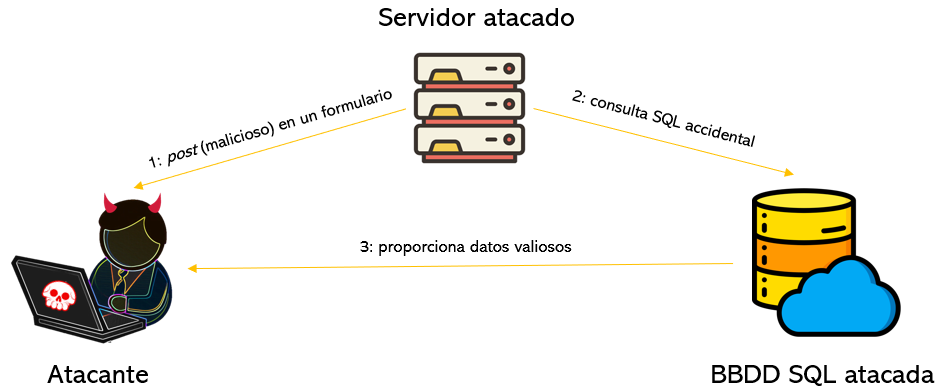
\includegraphics[scale=0.5]{../img/memoria/3_sqli}
\end{figure}

	\item \textbf{\textit{Cross-site request forgery} (CSRF)}: en este ataque se consigue que el navegador de un usuario legítimo envíe una petición HTTP maliciosa a un sitio objetivo. A ojos del servidor atacado, la petición es realizada por el usuario genuino (ya que sus \textit{cookies} son suplantadas), pero en realidad viene del atacante. El ataque puede originarse en forma de correos o páginas webs maliciosas, y el objetivo es una página legítima en la que el usuario ha tenido que iniciar sesión previamente. Las consecuencias (a parte de robo de información) son suplantaciones de identidad y se puede prevenir utilizando ciertas \textit{flags} de sesión en las \textit{cookies} o implementando \textit{tokens} CSRF~\cite{csrfatatus}.
	
	\begin{figure}[h]
		\caption[Ataques web: CSRF]{Infografía de un ataque CSRF.}
		\label{img:csrf}
		\centering
		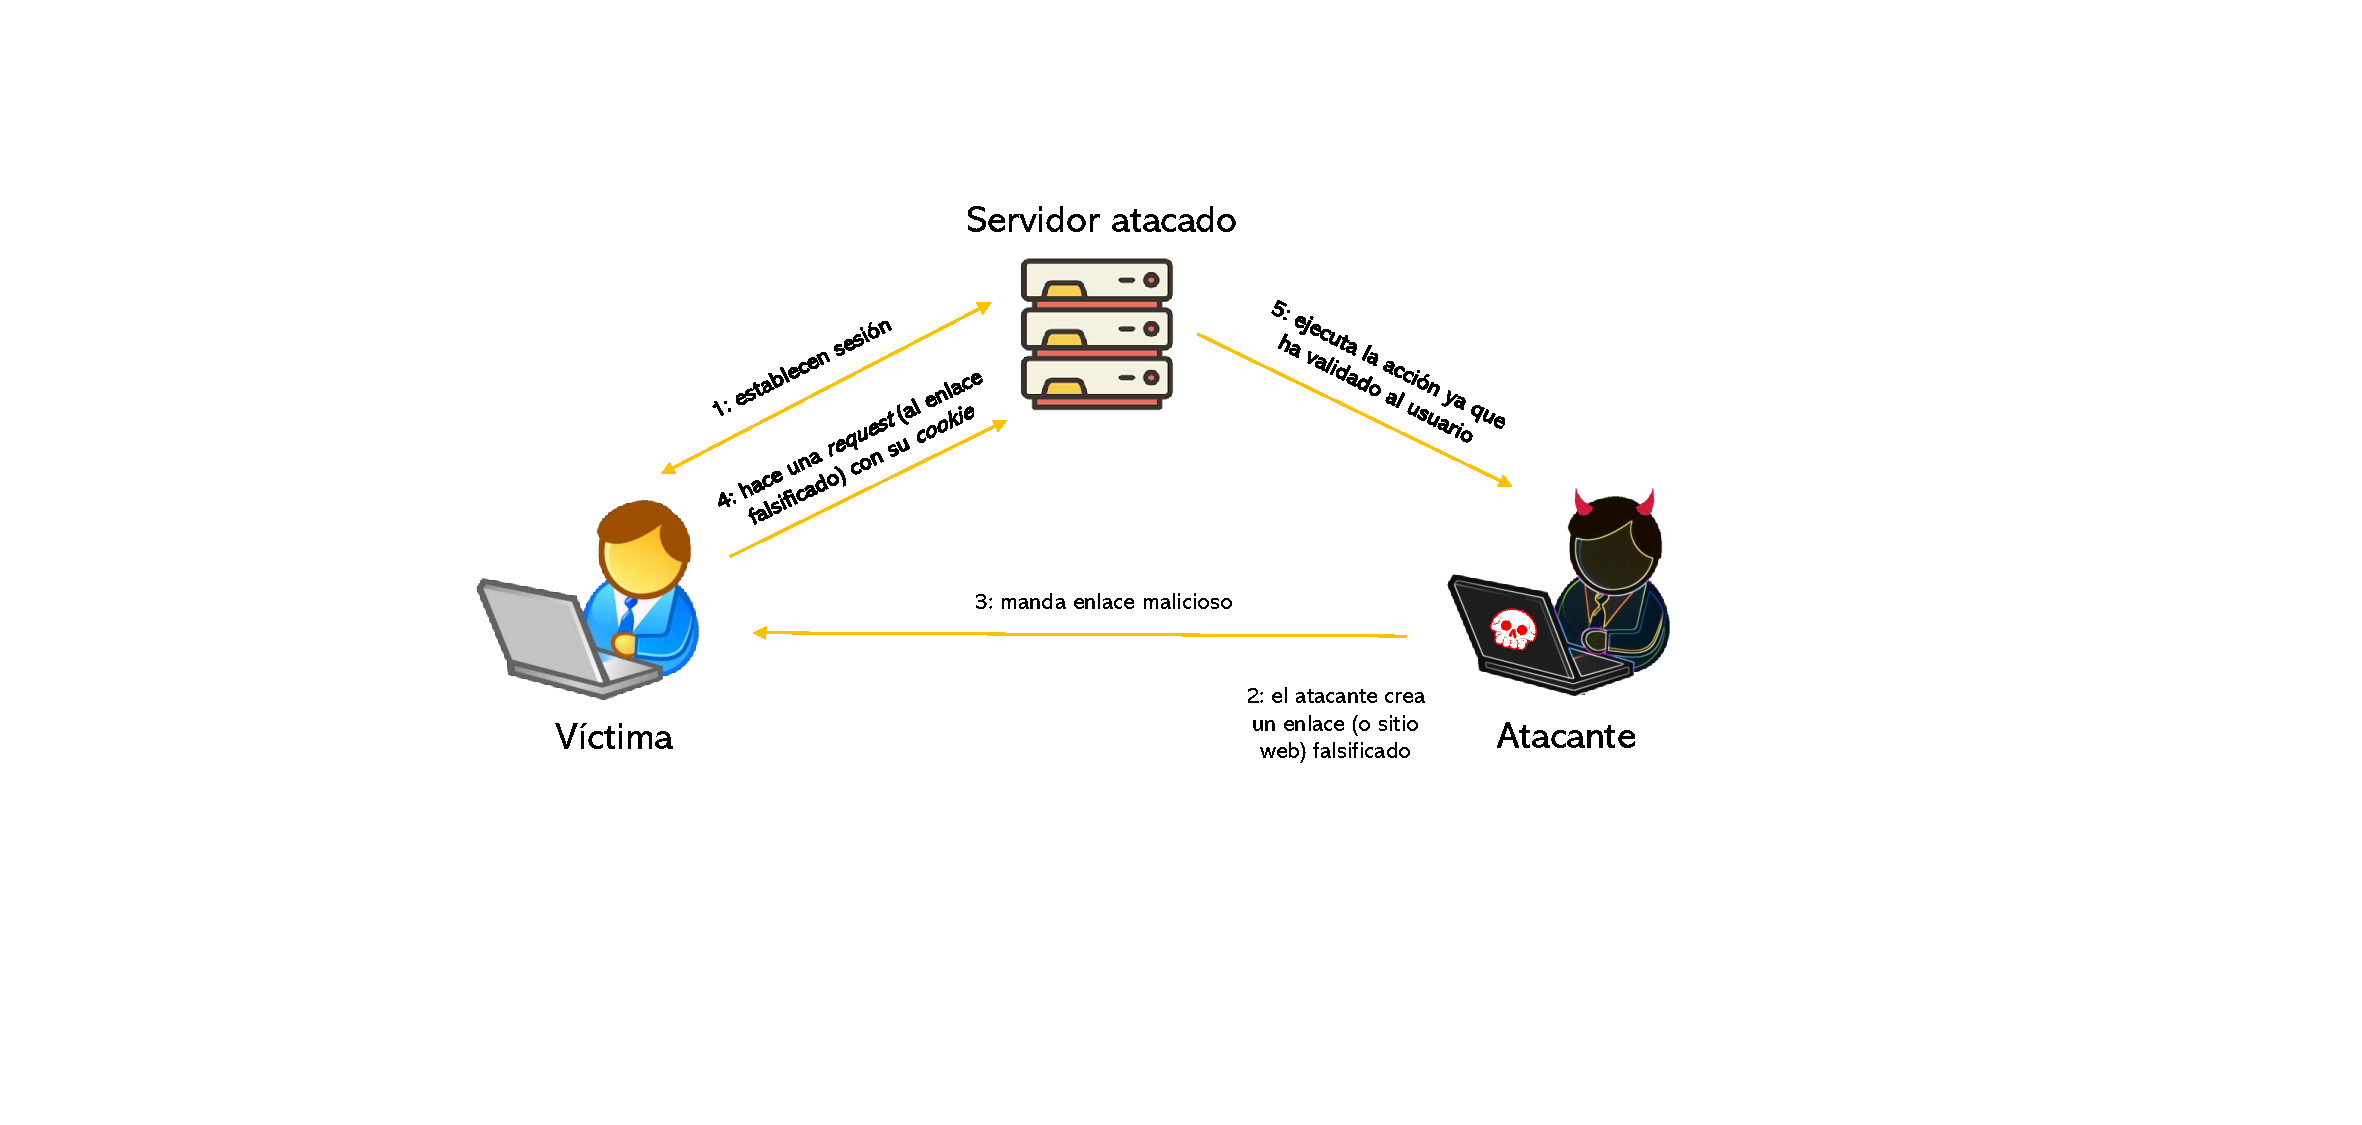
\includegraphics[scale=0.5]{../img/memoria/3_csrf}
	\end{figure}
	
	\item \textbf{\textit{Cross Site Scripting} (XSS)}: es uno de los ataques más populares existentes consistente en la inyección de código malicioso en el navegador de la víctima con el fin de robar información del usuario (\textit{cookies} o \textit{tokens} de sesión)~\cite{xssICM}. Suele estar realizado con \textit{JavaScript} y HTML (lado del cliente). Los dos escenarios más comunes son el XSS reflejado (la víctima recibe un enlace y se ejecuta código malicioso en su navegador) y el XSS almacenado (el \textit{script} malicioso se guarda en el servidor de forma permanente y se ejecuta en todos los navegadores de todos los usuarios que visiten la web)~\cite{xssDibus}.
	
	\begin{figure}[h]
		\caption[Ataques web: XSS]{Infografía de un ataque XSS.}
		\label{img:xss}
		\centering
		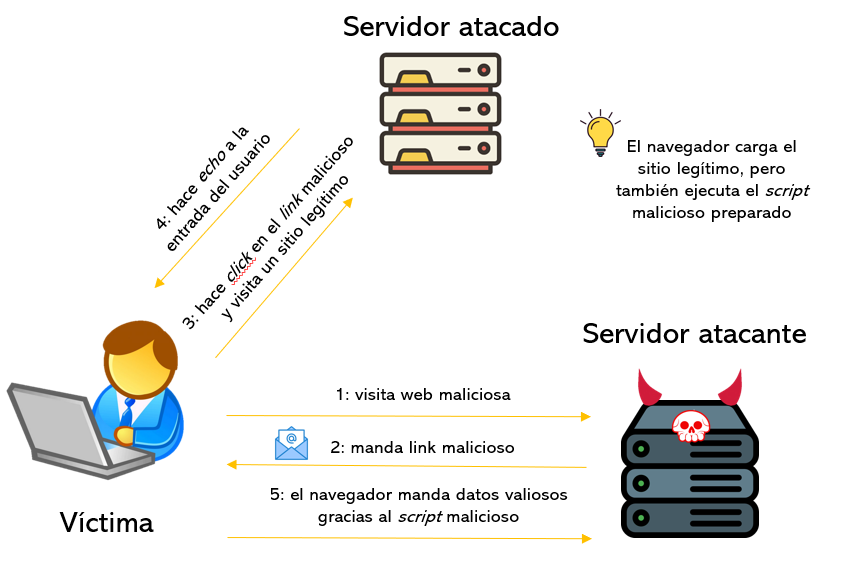
\includegraphics[scale=0.35]{../img/memoria/3_xss}
	\end{figure}
\end{itemize}

La principal diferencia entre XSS y CSRF es que XSS es un ataque <<de dos vías>> (permite al atacante ejecutar código, recibir respuestas y reenviarlas) y CSRF es de <<una vía>> (el atacante sólo puede lanzar una petición HTTP corrupta), de forma que el alcance de CSRF es limitado, mientras que XSS permite al atacante realizar prácticamente lo que desee. Además, XSS no necesita que se haya iniciado sesión previamente para tener éxito~\cite{xssVsCSRF}.

\section{Ataques a sistemas de recomendación}

Los ataques a los sistemas de recomendación (generalmene denominados \textit{shilling attacks}~\cite{mingdan2018ShillingAttacksAReview} o \textit{profile injection attack}~\cite{Mobasher2006Thesis}) tienen como objetivo manipular las sugerencias que propone un determinado algoritmo para conseguir que un cliente se incline hacia un elemento deseado. Esta alteración del sistema se consigue inyectando perfiles falsos.

Múltiples estudios se han centrado en formalizar las características de estos ataques con el fin de detectarlos. Entre ellas se encuentran~\cite{mingdan2018ShillingAttacksAReview}:

\begin{itemize}
	
	\item \textbf{Intención:} normalmente, se pretende manipular la opinión general acerca de un elemento (ya sea para bien o para mal). Según el objetivo se pueden diferenciar dos tipos de ataques: \textit{push attacks}, que pretenden hacer un objeto más atractivo o \textit{nuke attacks}, cuya intención es la contraria. En caso de que el atacante no busque alterar la opinión acerca de un producto sino restar credibilidad a un sistema (mediante valoraciones aleatorias), se habla de \textit{random vandalism}~\cite{Burke2015RobustCollaborative}.
	
	\item \textbf{Fuerza:} la calidad de los ataques se mide teniendo en cuenta el tamaño del relleno (número de valoraciones asignadas a un perfil atacante, que suele rondar entre el 1 y el 20\% del total de los ítems~\cite{mingdan2018ShillingAttacksAReview}), correspondiente a la ecuación~\ref{eqn:filler_size}  y el tamaño del ataque (número de perfiles inyectados en el sistema, rondando entre el 1 y el 15\%), correspondiente a la ecuación~\ref{eqn:attack_size} .
	
	\begin{equation}\label{eqn:filler_size} Filler size = \frac{|I_a|}{|I|}\end{equation}
	
	\begin{equation}\label{eqn:attack_size} Attack size = \frac{|U_a|}{|U_g|}\end{equation}
	
	\item \textbf{Coste:} se distinguen dos tipos: \textit{knowledge-cost}, que hace referencia al coste de construir perfiles y \textit{deployment-cost}, que es el número de perfiles que se deben inyectar para conseguir un ataque efectivo~\cite{Mobasher2006Thesis}.
	
\end{itemize}

\subsection{Tipos de ataques}

En la actualidad se distinguen multitud de ataques distintos. Con el fin de formalizarlos matemáticamente, se han establecido ciertos conjuntos de interés dependiendo de los ítems que contengan~\cite{zhou2021SemisupervisedRecommendationAttack}.

\begin{itemize}
	
	\item \textbf{$I_S$:} conjunto de ítems seleccionados para recibir un tratamiento especial (puede ser vacío).
	\item \textbf{$I_F$:} conjunto de ítems seleccionados para <<rellenar>>.
	\item \textbf{$I_0$:} conjunto de ítems pertenecientes al sistema de recomendación sin valorar.
	\item \textbf{$I_t$:} conjunto de ítems objetivo.
	
\end{itemize}


\subsubsection{Ataques básicos}

Se distinguen dos tipos: \textit{random attack} y \textit{average attack}~\cite{mingdan2018ShillingAttacksAReview}. Ambos tienen parámetros y características muy similares, como se muestra en la tabla \ref{tabla_descripcion_ataques_basicos}. La principal diferencia reside en que el \textit{average attack} es mucho más potente debido a que cuenta con mayor información acerca del sistema: las valoraciones a los ítems de relleno siguen una distribución $\mathcal{N}(\mu_i,\,\sigma_i)$, en lugar de $\mathcal{N}(\mu,\,\sigma)$. Es decir, la valoración para un determinado ítem se adecúa a la distribución concreta de ese ítem en lugar de a la de todo el \textit{dataset}.


\begin{table}
\small
\begin{centering}

		\begin{tabular}{@{}p{5em} p{2em} p{14em} p{2em} p{7em}@{}}
		\toprule
		\textbf{Modelo} & $\mathbf{I_S}$ & \textbf{Valoración} $\mathbf{I_F}$ & \hfil $\mathbf{I_0}$ & \textbf{Valoración} $\mathbf{I_t}$\\ 
		\midrule
	
		Random & $\emptyset$ & Aleatoria siguiendo una distribución normal definida por todas las valoraciones para todos los ítems del sistema $\mathcal{N}(\mu,\,\sigma)$. & \hfil $\emptyset$ & máxima o mínima \\\\
		
		Average & $\emptyset$ & Aleatoria siguiendo una distribución normal definida por las otras valoraciones para ese ítem en concreto $\mathcal{N}(\mu_i,\,\sigma_i)$. & \hfil $\emptyset$ & máxima o mínima\\
		\bottomrule
		\end{tabular}
	
\end{centering}
\caption[Sistemas de recomendación: ataques básicos]{Descripción de los ataques básicos.~\cite{zhou2021SemisupervisedRecommendationAttack}}
\label{tabla_descripcion_ataques_basicos}	
\end{table}


\subsubsection{Ataques con poco conocimiento del sistema}

Los más populares son \textit{bandwagon attack} (o \textit{popular attack}) y \textit{segment attack}. Sus principales rasgos se ilustran en la tabla \ref{tabla_descripcion_ataques_poco_con}.

La principal característica del \textit{bandwagon attack} es que el conjunto $I_S$ ya no está vacío, sino que contiene algunos de los ítems más populares de la base de datos~\cite{zhou2021SemisupervisedRecommendationAttack}. Estos ítems recibirán también la máxima puntuación posible, de forma que ya no sólo se puntúa el conjunto objetivo. Existe una variante de este ataque llamada \textit{reverse bandwagon attack}, cuyo objetivo es hacer \textit{nuke}, es decir, $I_S$ contiene los ítems menos populares y reciben la puntuación mínima (junto con $I_t$).

En el \textit{segment attack}, se realiza un pequeño <<estudio de mercado>> y se introduce en $I_S$ ítems en los que estaría interesado un usuario que fuese a valorar también $I_t$ (de forma que el ataque es más realista).

\begin{table}
\small
\begin{centering}
	
		\begin{tabular}{@{}p{5em} p{8em} p{8em} p{2em} p{7em}@{}}
			\toprule
			\textbf{Modelo} & $\mathbf{I_S}$ & \textbf{Valoración} $\mathbf{I_F}$ & \hfil $\mathbf{I_0}$ & \textbf{Valoración} $\mathbf{I_t}$\\ 
			\midrule
			
			Bandwagon (average) & Ítems populares (valoración máxima) o ítems desfavorecidos (puntuación mínima) (reverse) & Aleatoria siguiendo una distribución normal definida por las otras valoraciones para ese ítem en concreto $\mathcal{N}(\mu_i,\,\sigma_i)$. & \hfil $\emptyset$ & máxima o mínima (reverse) \\\\
			
			Bandwagon (random) & Ítems populares (valoración máxima) o ítems desfavorecidos (puntuación mínima) (reverse) & Aleatoria siguiendo una distribución normal definida por todas las valoraciones para todos los ítems del sistema $\mathcal{N}(\mu,\,\sigma)$. & \hfil $\emptyset$ & máxima o mínima (reverse) \\
			\bottomrule
		\end{tabular}

\end{centering}
\caption[Sistemas de recomendación: ataques con poco conocimiento]{Descripción de los ataques con poco conocimiento del sistema.}
\label{tabla_descripcion_ataques_poco_con}
\end{table}


\subsubsection{Ataques con gran conocimiento del sistema}

Este tipo de ataques resulta menos relevante que los anteriores debido a la dificultad de su ejecución. En la mayoría de los casos, se necesita una gran cantidad de información, siendo poco realista que se produzca una situación de estas características en la realidad.

Por ejemplo, el llamado \textit{perfect knowledge attack}~\cite{Mobasher2006Thesis} basa su efectividad en reproducir la distribución exacta de la base de datos real (exceptuándo los ítems objetivos). El \textit{sampling attack} construye los perfiles a inyectar basándose en una muestra de perfiles reales~\cite{mingdan2018ShillingAttacksAReview}.

Como se puede intuir, conocer datos estadísticos exactos sobre una base de datos o metadatos asociados a perfiles de usuarios es poco realista (cada vez menos debido a las mayores medidas de seguridad) y por lo tanto estos ataques resultan meramente teóricos.

\subsubsection{Ataques ofuscados}

Los ataques ofuscados~\cite{mingdan2018ShillingAttacksAReview} se basan en intentar <<camuflar>> los perfiles inyectados haciéndolos pasar por reales. Algunas de las características de su implementación se pueden consultar en la tabla \ref{tabla_descripcion_estrategias_ofuscación}.

El ataque de \textit{noise injection} introduce a los conjuntos $I_S$ e $I_F$ un <<ruido>> (número aleatorio que sigue una distribución Gaussiana) multiplicado por una constante $\alpha$. \textit{Target shifting} incrementa (o decrementa) en una unidad la valoración de $I_t$ con el fin de crear diferencias entre ataques similares sin influir excesivamente el resultado y el \textit{Average over popular items (AOP)} pretende ofuscar el \textit{average attack} cambiando la forma de selección de $I_F$ (en lugar de seleccionar los ítems del conjunto total de la colección, se seleccionan los $X\%$ ítems más populares).

\begin{table}
\small
\begin{centering}
	
		\begin{tabular}{@{}p{10em} p{20em}@{}}
		\toprule
		\textbf{Modelo} & \textbf{Estrategia de ofuscación}\\ 
		\midrule
			
		Noise Injection & $\forall i \in I_F \cup I_S: R_i = r_i + aleatorio * \alpha$\\
		Target Shifting & $\forall i \in I_F \cup I_S: R_i = r_i; I_T:$ $r_{max}-1$ o $r_{min}+1$\\
		AOP & $I_F$ escogido del top ítems más populares.\\
			
		\bottomrule
		\end{tabular}

\end{centering}
\caption[Sistemas de recomendación: estrategias de ofuscación]{Descripción de las estrategias de ofuscación.}	\label{tabla_descripcion_estrategias_ofuscación}
\end{table}

\subsubsection{Otros tipos de ataques}

Además de los ataques previamente ilustrados, existen otros con objetivos más diversos o estrategias distintas. El anteriormente mencionado \textit{random vandalism} (cuya intención únicamente es degradar la calidad del recomendador para causar descontento entre los usuarios) pertenece a esta categoría. Se pueden distinguir, además, ataques basados en copiar comportamientos de usuarios influyentes (modelo \textit{PUA} (\textit{Power User Attack})) o ítems poderosos (modelo \textit{PIA} (\textit{Power Item Attack}))~\cite{mingdan2018ShillingAttacksAReview}. Sin embargo, son menos populares.


\section{\textit{Phishing}}

\subsection{TF-IDF}

TF-IDF es un algoritmo que pretende definir la importancia que tiene una determinada palabra dentro de un documento teniendo en cuenta la relación que pueda tener con otros documentos dentro del mismo cuerpo~\cite{tfidfmarius2020}. Es decir, es una especie de <<puntuación>> para cada palabra del texto que aumenta cada vez que hay una ocurrencia, pero disminuye gradualmente cada vez que aparece en el resto de la colección. Por este motivo, puede ser realmente útil a la hora de extraer \textit{keywords}~\cite{cantinatfidf}. Se basa en dos principios:

\begin{enumerate}
	\item Una palabra que aparezca con mucha frecuencia en un documento tiene especial importancia para el mismo, por lo que es probable que el texto tenga relación con esa palabra.
	\item Una palabra que aparezca repetidamente en varios documentos no sirve para identificar uno (o un pequeño subconjunto) en una colección (no sirve como \textit{keyword}), por lo que no es relevante para el mismo.
\end{enumerate}

Para calcular esta puntuación, se han de utilizar las ecuaciones facilitadas a continuación, donde $N$ es el número de documentos disponibles, $d$ es un documento en concreto, $D$ es la colección de todos los documentos y $w$ es una palabra dentro de un documento.

\begin{itemize}
	\item \textbf{TF}: la frecuencia de una palabra $w$ en un documento $d$ se calcula con la ecuación~\ref{eqn:tf}.
	
	\begin{equation}\label{eqn:tf} \textrm{tf(w,d)} = \log{(1 + f(w,d))} \end{equation}
	
	\item \textbf{IDF}: la frecuencia inversa de una palabra $w$ en la colección $d$ se calcula con la ecuación~\ref{eqn:idf}, aunque puede implementarse de otras maneras~\cite{tfidfsklearn2020} en función del peso que se quiera dar.
	
	\begin{equation}\label{eqn:idf} \textrm{idf(w,D)} = \log{(\frac{N}{f(w,D)})} \end{equation}
	
	\item \textbf{TF-IDF}: la puntuación TF-IDF se obtiene en combinación de las dos puntuaciones anteriores.
	
	\begin{equation}\label{eqn:tfidf} \textrm{tf-idf(w,d,D)} = tf(w,d) \times idf(w,D) \end{equation}
	
\end{itemize}














